%% !Mode:: "TeX:UTF-8"
\documentclass{mcmthesis}
%  \documentclass[CTeX = true]{mcmthesis}
\mcmsetup{tstyle=\color{red}\bfseries,%修改题号,队号的颜色和加粗显示,黑色可以修改为 black
        tcn = 2512625, problem = C, %修改队号,参赛题号
        sheet = true, titleinsheet = true, keywordsinsheet = true,
        titlepage = false, abstract = true}

% 代码块设置
    \usepackage{fontspec}
    \setmainfont{Charter} [
        Extension = .ttf,
        UprightFont = * Regular,
        BoldFont = * Bold, 
        ItalicFont = * Italic,
        BoldItalicFont = * Bold Italic
    ]
    \newfontfamily\consolasfont{Consola}[
        Extension = .ttf,
        UprightFont = *,
        BoldFont = *b,
        ItalicFont = *i,
          BoldItalicFont = *z
    ]

    \definecolor{bg}{rgb}{0.92,0.95,1.0} % Lighter blue fill
    \definecolor{borderblue}{rgb}{0.4,0.4,1.0} % Blue border
    \definecolor{commentcolor}{rgb}{0.4,0.85,0.4} % Softer green comment color

    \lstset{
        basicstyle=\consolasfont\footnotesize,  % Changed to use Consolas
        backgroundcolor=\color{bg},
        lineskip=1.5pt,
        frame=single,
        framesep=1mm,
        rulecolor=\color{borderblue}, % Blue border
        numbers=left,
        numberstyle=\small\color{gray}, % Changed from \tiny to \small
        keywordstyle=\color{blue},
        commentstyle=\color{green},
        commentstyle=\color{commentcolor}\itshape,
        stringstyle=\color{red},
        showstringspaces=false,
        breaklines=true,  % Ensure lines break within margins
        breakatwhitespace=true, % Allow breaking at whitespace
        prebreak=\raisebox{0ex}[0ex][0ex]{\ensuremath{\hookleftarrow}},
        postbreak=\raisebox{0ex}[0ex][0ex]{\ensuremath{\hookrightarrow}},
        escapeinside={(*@}{@*)},
        literate={-}{{\textendash}}1
    }
 
\usepackage{indentfirst}  %首行缩进,注释掉,首行就不再缩进。
\usepackage{lipsum}
\usepackage{wrapfig} % 图文绕排
\usepackage{enumitem} % 列表间距
\usepackage{caption} 

\captionsetup[figure]{justification=centering}
\captionsetup[table]{justification=centering}
 
% 设置全局段间距
\setlength{\parskip}{0.25em}

\setenumerate[1]{itemsep=1pt,partopsep=0pt,parsep=\parskip,topsep=2pt}
\setitemize[1]{itemsep=1pt,partopsep=0pt,parsep=\parskip,topsep=2pt}

% 调整浮动体参数
\setcounter{topnumber}{6}% 每页顶部最大浮动体数量
\setcounter{bottomnumber}{3}% 每页底部最大浮动体数量
\setcounter{totalnumber}{6}% 每页浮动体总数量
\renewcommand{\topfraction}{0.95}% 页面顶部浮动体比例
\renewcommand{\bottomfraction}{0.5}% 页面底部浮动体比例
\renewcommand{\floatpagefraction}{0.9}% 浮动体页比例
\renewcommand{\textfraction}{0.05}% 正文比例

\title{Mathematical Model for Prediction of Olympic Medal Counts}
\author{\small \href{https://www.latexstudio.net/}
  {\includegraphics[width=7cm]{mcmthesis-logo}}}
\date{\today}

\begin{document}
\begin{abstract}
    \par 
    Our research develops a robust framework for predicting medal counts at the 2028 Los Angeles Summer Olympics, grounded in an extensive analysis of historical data, and addresses three key tasks: forecasting medal distribution, evaluating the influence of elite coaching, and uncovering novel insights into Olympic medal dynamics.

    \textbf{Task 1} focuses on medal prediction through a \textbf{tier-based modeling approach}. Using \textbf{K-means clustering}, we classified countries into five tiers based on recent historical performance, tailoring prediction models to the unique dynamics of each group. With a \textbf{metaheuristic} algorithm, we optimized the feature selection process. \textbf{Regression techniques}, including LSBoost, XGBoost, random forests, etc., as well as optimizing algorithms, including SSA \cite{8}, DBO \cite{9}, SCA \cite{10}, etc., were implemented with the \textbf{TOPSIS} method used to identify the most effective model and algorithm. We also introduced \textbf{K-Fold algorithm} to split datasets into training, validating, and testing sets. Additionally, an analysis of the relationship between sports' global importance and medal distribution, using \textbf{Spearman's rank correlation coefficient}, confirmed the substantial benefits host countries derive, such as increased medal counts and event-specific advantages.
    
    \textbf{Task 2} explores the "Great Coach Effect" wherein elite coaches significantly influence national Olympic success. By analyzing \textbf{coaching transfers} and \textbf{performance trends}, we quantified the impact of high-caliber coaching on medal counts. \textbf{Regression analysis} revealed that this effect is particularly pronounced in \textbf{lower-tier/underperforming countries}, where elite coaching can lead to substantial improvements. Based on these findings, we recommend prioritizing the recruitment of top-tier coaches in countries with the potential for notable performance gains.
    
    \textbf{Task 3} delves into the original insights revealed from our model. Firstly, we explored the concept of \textbf{Global Sports Equity}, highlighting the significant impact of elite coaching on low-tier countries and recommending the sharing of coaching expertise to foster a more equitable global sports landscape. Secondly, we analyzed the \textbf{Host Country Effect}, observing substantial increases in medal counts for host nations and suggesting regulations to mitigate this advantage. Thirdly, we identified a \textbf{Time-Sensitive Element} in our prediction model, emphasizing the importance of recent match data in optimizing performance. Lastly, we discussed the \textbf{Granularity Effect} in prediction models, recommending a diversified participation strategy to maximize medal-winning opportunities. Our \textbf{sensitivity analysis} further confirmed the model's stability with respect to the number of estimators, ensuring robust prediction performance.
    
\begin{keywords}
    Olympics Medal Prediction; Regression Models; K-Fold; Optimizing Algorithm; Metaheuristic Algorithm
\end{keywords}

\end{abstract}
\maketitle
\tableofcontents
\newpage

\section{Introduction}
\subsection{Problem Background}
The Olympic medal table is a key focus for nations and fans, reflecting athletic success and national pride. Predicting medal counts is challenging due to complex factors like event types, host country advantages, and new competitors. This problem requires models based on provided datasets, including historical medal tables, event breakdowns, and athlete performance.

Traditional forecasting methods, like OLS regression and Poisson models, often lack accuracy, especially when the precise data of participants and events is absent. This problem emphasizes predicting medal breakthroughs for the introduction of new algorithms and projection strategies based on historical trends.

Meanwhile, the dynamic nature of sports, with evolving rules, emerging talents, and varying levels of investment in different countries, adds another layer of complexity. Our approach incorporates regression model techniques and tier-based modeling to address these challenges, aiming to provide more accurate and insightful predictions. Our model strives to capture the multifaceted influences on Olympic performance, offering a comprehensive tool for forecasting future medal counts.

\subsection{Literature Review}

Predicting Olympic medal counts has been a topic of interest for researchers across various fields, including economics, sociology, and sports science. Early studies, such as those by Ball (1972)\cite{1}, focused on identifying fundamental socioeconomic and demographic factors that influence a nation's medal count. Subsequent research, including work by Bernard and Busse (2004) and Xun Bian (2005) \cite{2, 3}, further explored the impact of political systems and hosting advantages on medal counts, finding that hosting the Games and having a centrally-planned economy can significantly enhance a country's performance. Recent advancements in statistical and machine learning techniques have led to more sophisticated models for predicting Olympic medals. Forrest et al. (2010) \cite{4} enhanced traditional regression-based models by including additional regressors such as public spending on recreation and the effects of future hosts.

Despite significant progress, predicting Olympic medals remains a complex task due to the interplay of numerous factors. Overall, the field has evolved from simple correlation-based models to sophisticated machine learning algorithms, with traditional socioeconomic factors remaining significant predictors of Olympic success.

\subsection{Our Work}

Our entire workflow is demonstrated in \textit{Figure~\ref{fig:ourwork}}.

\begin{figure}[htbp]
    \centering
    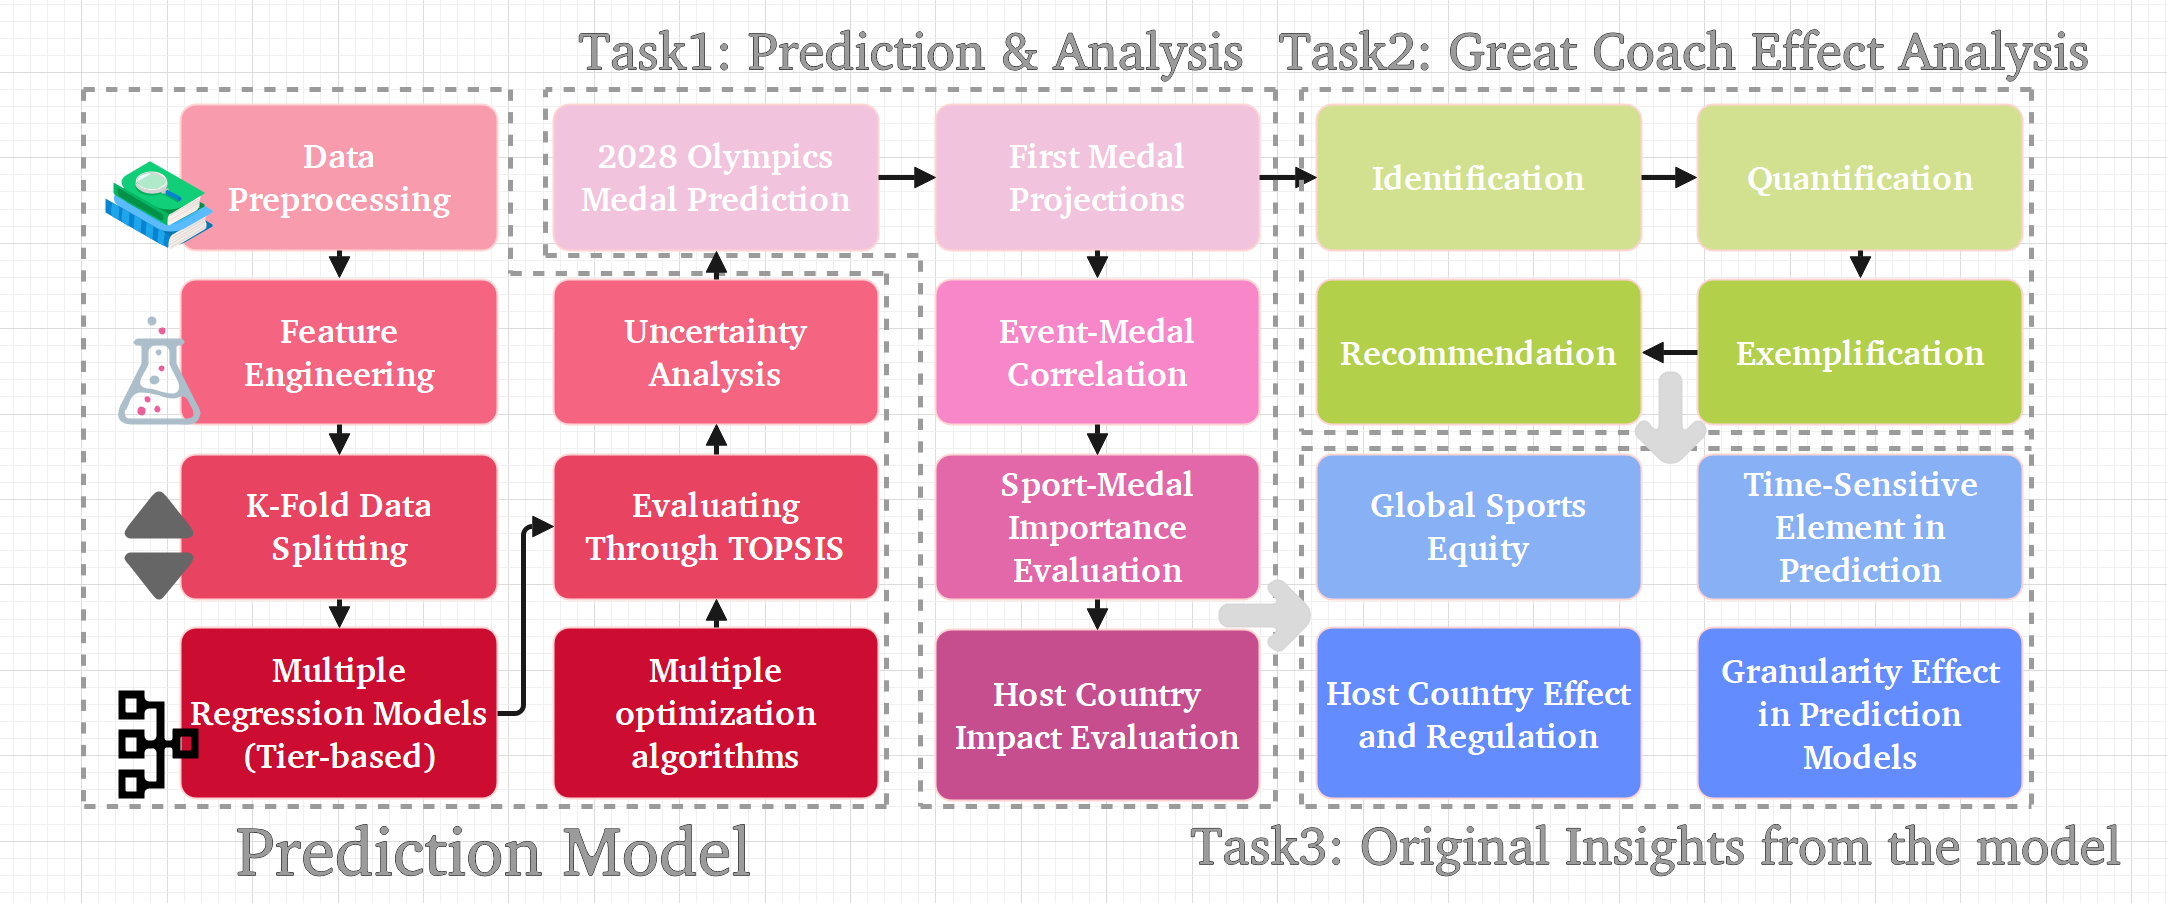
\includegraphics[width=1\textwidth]{pics/ourwork.png}
    \caption{Our entire workflow}
    \label{fig:ourwork}
\end{figure}

% As can be seen from the figure above, we have meticulously designed the model structure to seamlessly integrate various tasks and derive effective and sound conclusions.

% Due to the limitation of usable dataset, we cannot explore many of the aforementioned factors in detail. Instead, we focus on developing a model that predicts Olympic medal counts based on historical data and sport-specific information. Our model has the following features:

% \begin{enumerate}
%     \item A tier-based modeling strategy that classifies countries into five tiers based on their historical performance, allowing for more accurate predictions for countries with similar overall strengths.
%     \item A two-stage model that first predicts the number of medals won by each country in each sport, then aggregates these predictions to estimate the total medal count.
%     \item Trains and evaluates multiple models on the same dataset, and uses the best-performing model for prediction.
%     \item Quantifies the uncertainty in model predictions using Gaussian Probability Interval Prediction, providing upper and lower bounds for the estimated medal counts.
%     \item A sensitivity analysis that assesses the impact of different factors on medal counts and identifies key drivers of success.
% \end{enumerate}

\section{Assumptions and Justifications} 

\subsection{Historical Consistency}
    
    We assume that historical trends in medal counts are consistent with future performance. This assumption is at the heart of our model and is supported by previous research on the predictability of Olympic medal counts \cite{4,5,7}.
\subsection{Comprehensive national power's great impact on medal count}
    
    It's been widely acknowledged that a country's comprehensive national power, including economic, political, and social factors, has a significant impact on its Olympic performance \cite{1,2,3,7}. Because the provided dataset doesn't include the detailed information of these factors like GDP, we manually categorize countries into different tiers based on their historical medal counts, which is a good proxy for their comprehensive national power. For more detail, see Data Preprocessing part.
\subsection{Host Country Advantage}
    
    We assume that host countries have a competitive advantage due to factors such as home crowd support and familiarity with the venues.
\subsection{Time Proximity}
    
    We assume that only the recent Olympic data is relevant for predicting future medal counts. This assumption is based on the idea that recent performance trends and current athlete conditions are more indicative of future outcomes than older data. Therefore, our model primarily focuses on the last few Olympic Games to ensure the predictions are based on the most relevant and up-to-date information.
\subsection{Sport as minimal granularity}
    
    We assume that using sport as the minimal granularity of data is the best for predicting medal counts, namely, we predict the medal outcome of each sport and sum them up to obtain the projected medal count for each country. This is justified by our trial-and-error process, which found that using event or individual athlete as the minimal granularity of data leads to overfitting and poor generalization. Granularity too small leads to higher randomness and fewer samples for each unit, and neither of them are beneficial for the accurate prediction of medal counts in the next Olympic Games. Therefore, we use sport as the minimal granularity of data in our model.

\section{Notations and Definitions}

Our model employs a range of notations and definitions to facilitate the analysis and prediction of Olympic medal counts. These notations are summarized in \textit{Table~\ref{tab:notations}}.

\newpage

\begin{table}[h!]
    \centering
    \begin{tabular}{ccc}
        \toprule
        \textbf{Notation} & \textbf{Definition} \\ 
        \midrule
        $C_i$ & Country $i$, $i \in \{1, 2, \ldots, N\}$; $N$: total number of countries. \\
        $E_j$ & Event $j$, $j \in \{1, 2, \ldots, M\}$; $M$: total number of events. \\
        $S_k$ & Sport $k$, composed of related events $E_j$, \\
             & $k \in \{1, 2, \ldots, L\}$; $L$: total number of sports. \\
        $m_{i,j}$ & Medals won by country $C_i$ in event $E_j$ from 2012 to 2024. \\
        $M_i$ & Total medals won by country $C_i$, $M_i = \sum_{j=1}^M m_{i,j}.$ \\
        $w_{i,j}$ & Importance of event $E_j$ for country $C_i$, $w_{i,j} = \frac{m_{i,j}}{M_i}.$ \\
        $W_j$ & Global importance of event $E_j$, $W_j = \sum_{i=1}^N w_{i,j}.$ \\
        $I_k$ & Global importance of sport $S_k$, $I_k = \sum_{j \in S_k} W_j.$ \\
        $S_{xx}$ & Sum of square deviation of $x$, $S_{xx} = \sum_{i=1}^n (x_i - \bar{x})^2.$ \\
        \bottomrule
    \end{tabular}
    \caption{Summary of notations and definitions}
    \label{tab:notations}
\end{table}


\section{Data Preprocessing}
% remember to mention some details
% 1. event/sport name changed over the course of time
% 2. some special years like 1906, when an unofficial Olympic Games was held. We need to exclude this year from our analysis.
% 3. event name ambiguity, e.g. 500+ events named "Men" and "Women"
\subsection{Early Attempts: Athlete-based Prediction}
First, we ruled out the approach of predicting medal counts based solely on the historical total medal data of countries, as this method is both logically flawed and overly simplistic. Given that the most detailed dataset provided includes information on individual Olympic competitors, their respective sports, events, and results, it is a natural and more precise approach to base medal predictions on the performance of individual athletes participating in specific events.

Furthermore, we aimed to incorporate the host country as a training feature by matching it to the competing country, while the dataset only provided the host city. Recognizing the National Olympic Committee (NOC) code as a standardized and uniform identifier for countries, we created a dataset named "City\_NOC.csv" to serve as a dictionary containing all Olympic host cities and their corresponding NOC codes. Using this dictionary, we developed a Python script to add a new column, "host\_NOC", to the dataset while removing the original "City" column. Additionally, we excluded all data from the 1906 Olympics, as it was an informal event and disrupted the four-year cycle traditionally followed by the Olympic Games.

To further enhance data quality, we normalized medal counts by dividing them by their corresponding team sizes \AIcite{AI2} using a Python script. This normalization step ensured that the data accounted for the nature of team events, eliminating biases caused by repeated medal counts. We subsequently created a training dataset consisting of individual participants as rows and their corresponding medals earned and host NOC for each year as columns.

\subsection{Current Method: Sport/Event Oriented Data Preprocessing}

Despite these efforts, the athlete-based prediction results were significantly lower than the actual medal counts. This discrepancy likely stems from the instability of individual performances and the reality that most athletes do not participate in multiple Olympic Games, let alone win multiple medals. Consequently, we shifted to a more aggregated and macroscopic approach, categorizing data by country(NOC) and sport. We anticipated this method would yield more stable and reliable predictions.

To refine the dataset further, we addressed an issue where substitutes were included in the list of athletes, rendering team size unsuitable for normalizing medal counts. To resolve this, we removed columns such as Name, Sex, Team, and Event, which were irrelevant to the country- and sport-based approach. We then eliminated duplicate rows to create a cleaned dataset, "summerOly\_medal\_norepeat.csv", which contained all medals without repetition or omission.

Moreover, we recognized "No Medal" as a potential indicator of a country's capability in specific events. Countries participating in a sport are likely to perform better than those that do not. Therefore, we introduced a "No Medal" column as a parallel feature alongside the Gold, Silver, and Bronze medal counts for model training.

To enhance prediction accuracy, we employed the K-means clustering algorithm to classify all participating countries into 5 distinct tiers based on their historical medal counts. As a result, Tier 5, the highest tier, comprised only the United States (USA) and China (CHN), which dominated in gold and total medal counts. Tier 4 and Tier 3 were identified based on a significant gap in gold medal counts, with Italy (38) marking the boundary between the two tiers and New Zealand (27) serving as the lower boundary of Tier 3. Tier 2 and Tier 1 were marked by total medal counts of 14 and 6, respectively. This tier-based categorization allowed for a more structured and nuanced analysis of countries' performance trends.

\subsection{Cumulative Medal-Winning Countries by Olympic Year}
Problem 1.2 requires projecting how many countries will earn their first medal in the next Olympics. To address this, we utilized the "summerOly\_medal\_norepeat.csv" dataset that was prepared earlier. A new column, "Medal", was added to the dataset, representing the sum of the "Gold", "Silver", and "Bronze" columns to indicate whether a given row corresponds to a medal-winning entry.

Subsequently, we developed a Python script to calculate the year in which each country earned its first medal. For countries that have not yet won any medals, the "Year" column was assigned the value 2028 to reflect the next Olympic cycle. Following this, another Python script was created to calculate the cumulative number of countries that had won medals up to each Olympic year. This cumulative count served as the foundational data for time series projection.

\section{Establishing the Model}

In this section, we outline the process of developing a regression-based model to predict medal counts (Gold, Silver and Bronze medals) for each country in the Los Angeles 2028 Summer Olympics. Our methodology accounts for historical performance, and hosting effects. The proposed approach includes estimates of uncertainty, prediction intervals, and measures of model performance.

Thanks to the nature of this problem being inherently correlated to chronological projection and the provided data being complete with regard of countries, sports, events and individual athletes, we adopt time series analysis and regression models to predict medal counts for the 2028 Los Angeles Olympics.

To specify, we adopt a tier-based modeling strategy, aligning with the classification to be established in Task 1 - Subtask 3. Countries are grouped into five tiers based on their historical performance. Separate regression models are trained for each tier to capture the unique dynamics of countries within the same tier. The methodology involves the following steps:

\subsection{Data Loading \& Transformation}

\begin{itemize}
    \item \textbf{Loading:} We use data from the most recent eight Olympic Games, including information on hosting nations and medal counts (Gold, Silver, and Bronze) for each participating country.
    \item \textbf{Transformation:} Hosting nation information is one-hot encoded to introduce categorical variables. To address class imbalance, the SMOTE (Synthetic Minority Oversampling Technique) algorithm is applied, generating synthetic samples for underrepresented classes and balancing the dataset.
\end{itemize}

\begin{wrapfigure}{r}{8cm}  %这是图文混排的环境
    \centering
    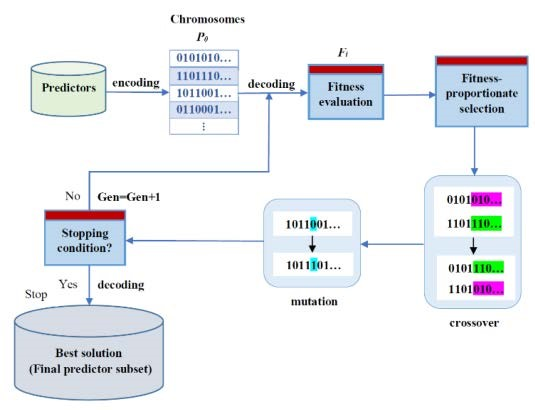
\includegraphics[width=0.9\linewidth,height=6cm]{pics/Multi-Agent_Optimization_Algorithm.jpg}
    \caption{Mechanism of metaheuristic algorithm}
    \label{fig:metaheuristic_algorithm}
\end{wrapfigure}

\subsection{Feature Engineering}

Features are selected and optimized using metaheuristic algorithm to determine the most effective combinations. Like the image showed, this process involves transforming the feature selection problem into a binary optimization problem, where:
\begin{itemize}
    \item A value of 0 indicates the exclusion of a feature.
    \item A value of 1 indicates the inclusion of a feature.
\end{itemize}
A regression model is trained iteratively with different feature combinations, and the performance of each combination is evaluated. 


\subsection{Data Splitting}

Given the relatively small dataset size, we adopt k-fold cross-validation to split the data into training, validation, and testing subsets. This approach ensures that the model is evaluated robustly across multiple splits of the data.

\subsection{Model Training}

We train several regression models on the training set, including: LSBoost, XGBoost, Multivariate Linear Regression, Gaussian Regression, Decision Tree, Random Forest. Each model is trained using the training set and evaluated on the validation set to determine the optimal hyperparameters.

\subsection{Model Evaluation}

The performance of each model is assessed on the test set using the following metrics:Mean Absolute Error (MAE), Mean Absolute Percentage Error (MAPE), Mean Squared Error (MSE), Root Mean Squared Error (RMSE), Coefficient of Determination ($R^2$)

The evaluation result is shown in \textit{Figure~\ref{fig:model_comparison}}. From the result we can see that each medal type can have very different best models. This phenomenon also vouches for the veracity of our tier-based modeling strategy.

%! TODO: insert the figure here
% \begin{figure}[htbp]
%     \centering
%     % First row
%     \begin{minipage}[t]{0.48\textwidth}
%         \centering
%         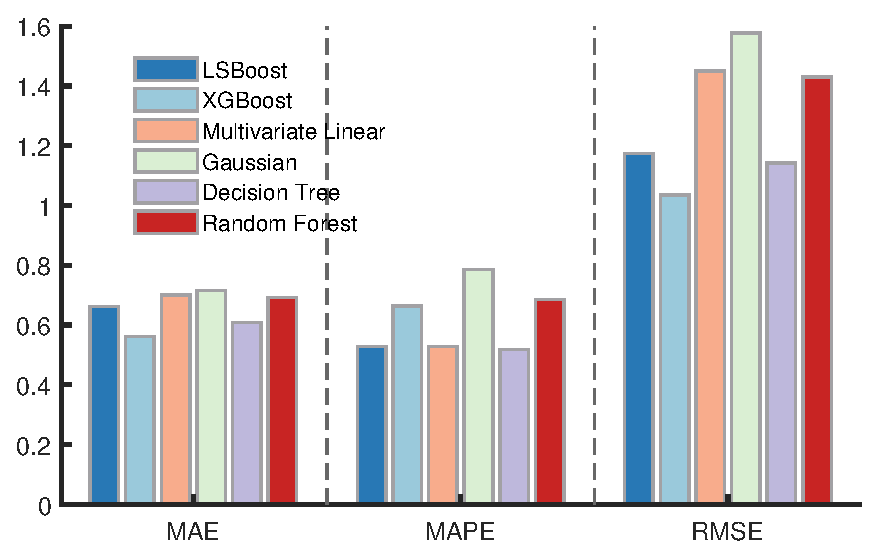
\includegraphics[width=2.2in, keepaspectratio]{pics/multi-regression-compare.eps}
%         \label{fig:performance1}
%     \end{minipage}
%     \hfill

%     \begin{minipage}[t]{0.48\textwidth}
%         \centering
%         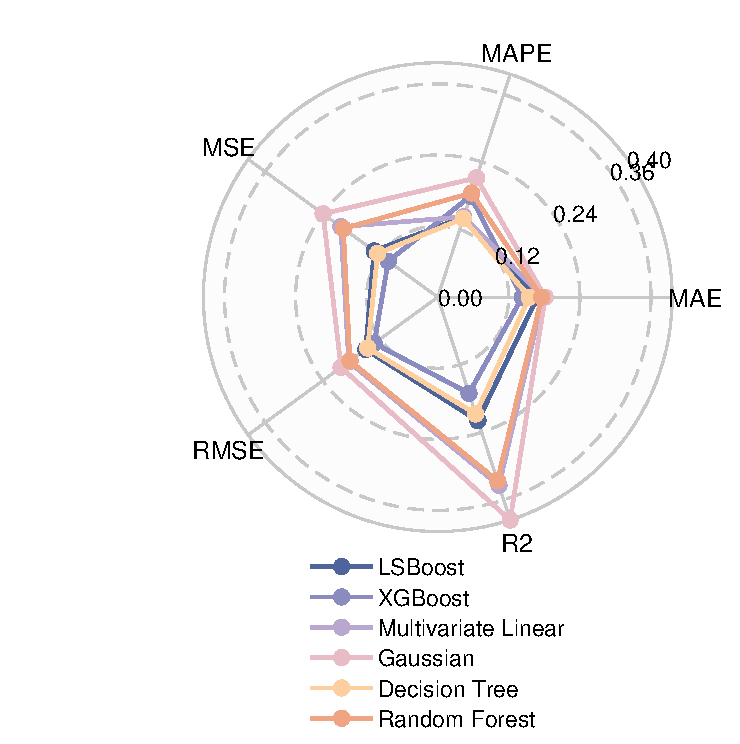
\includegraphics[width=2.2in, keepaspectratio]{pics/multi-regression-compare-5.eps}
%         \label{fig:performance3}
%     \end{minipage}
    
%     \vspace{0.4cm} % Space between rows
    
%     % Second row
%     \begin{minipage}[t]{0.48\textwidth}
%         \centering
%         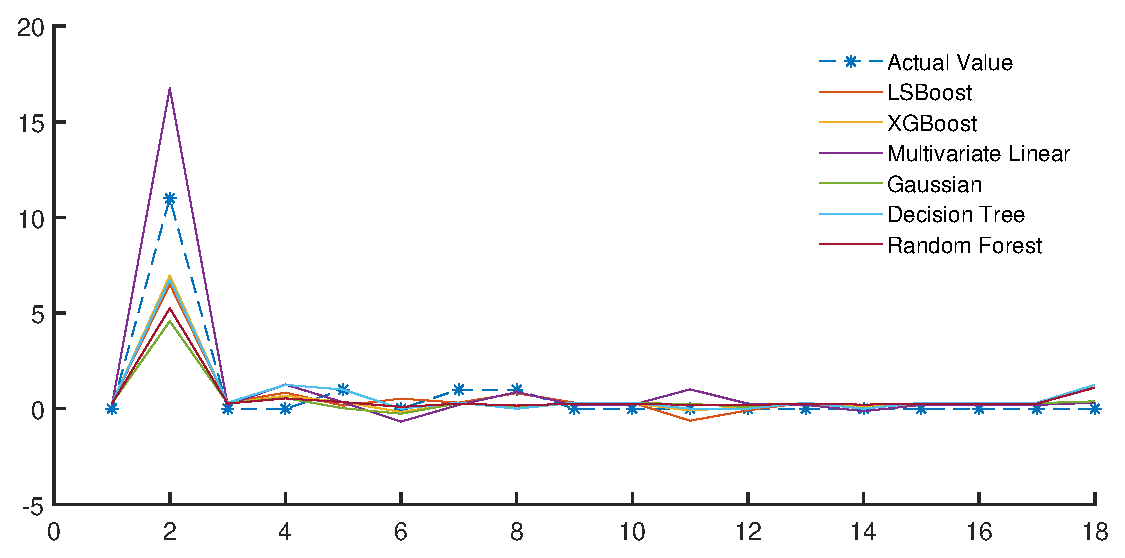
\includegraphics[width=2.2in, keepaspectratio]{pics/multi-regression-compare-3.eps}
%         \label{fig:performance4}
%     \end{minipage}
%     \hfill
%     \begin{minipage}[t]{0.48\textwidth}
%         \centering
%         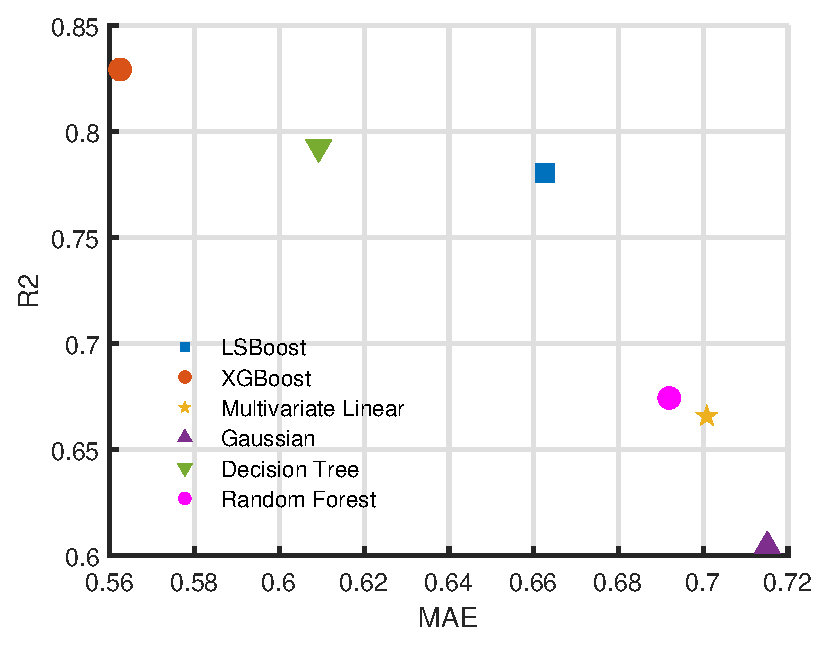
\includegraphics[width=2.2in, keepaspectratio]{pics/multi-regression-compare-2.eps}
%         \label{fig:performance2}
%     \end{minipage}
    
%     \caption{Performance comparison of different regression models for predicting Tier 1 Gold medal prediction model.}
%     \label{fig:model_comparison}
% \end{figure}
\begin{figure}[!htbp]
    \centering
    % First row
    \begin{minipage}[t]{0.58\textwidth}
        \centering
        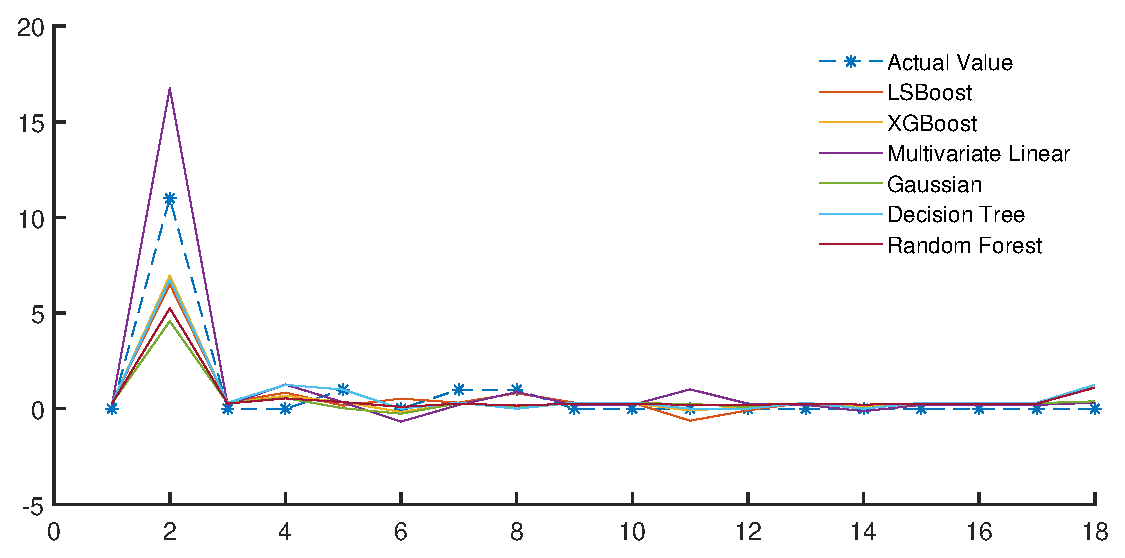
\includegraphics[width=\textwidth, keepaspectratio]{pics/multi-regression-compare-3.eps}
        % \caption{(a)} % Subfigure label
        % \label{fig:performance1}
    \end{minipage}
    \hfill
    \begin{minipage}[t]{0.4\textwidth}
        \centering
        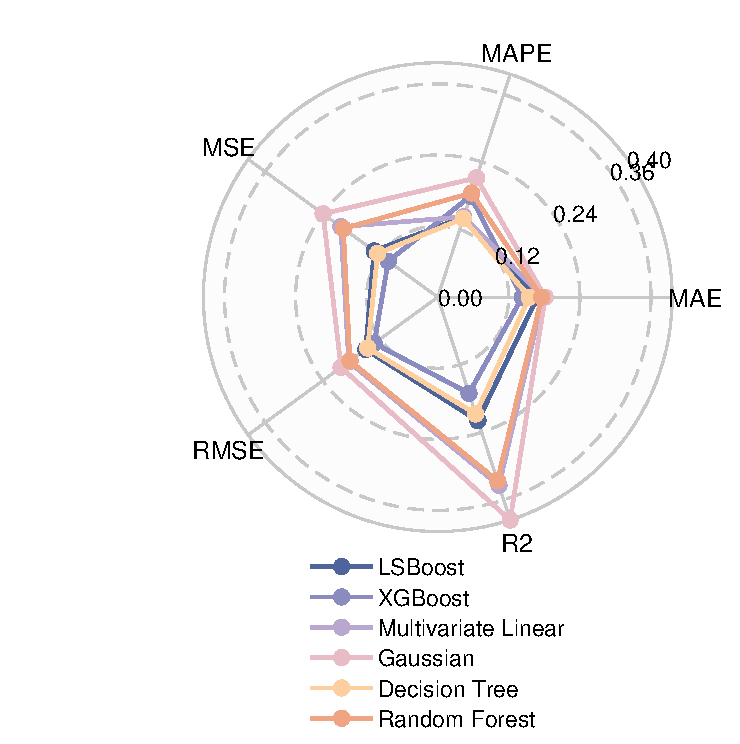
\includegraphics[width=\textwidth, keepaspectratio]{pics/multi-regression-compare-5.eps}
        % \caption{(b)} % Subfigure label
        % \label{fig:performance3}
    \end{minipage}
    
    \vspace{0.2cm} % Space between rows

    % Second row
    \begin{minipage}[t]{0.52\textwidth}
        \centering
        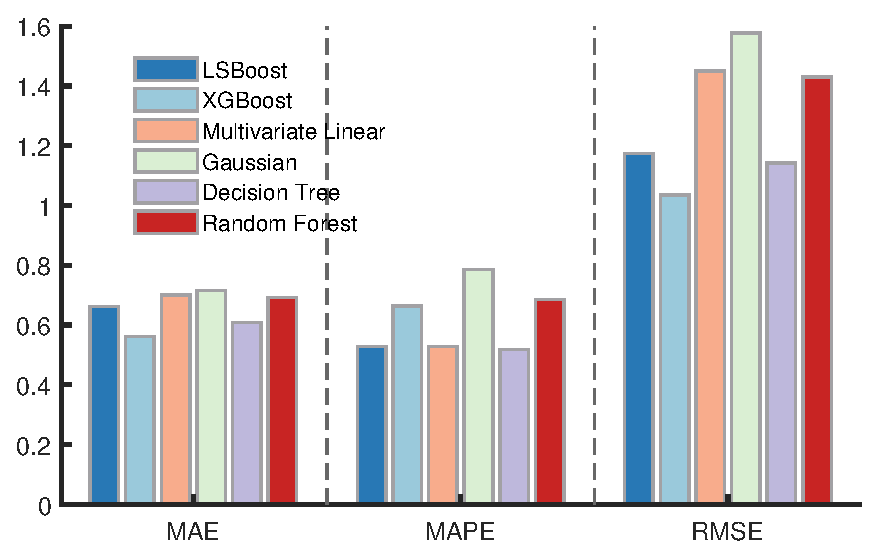
\includegraphics[width=\textwidth, keepaspectratio]{pics/multi-regression-compare.eps}
        % \caption{(c)} % Subfigure label
        % \label{fig:performance4}
    \end{minipage}
    \hfill
    \begin{minipage}[t]{0.44\textwidth}
        \centering
        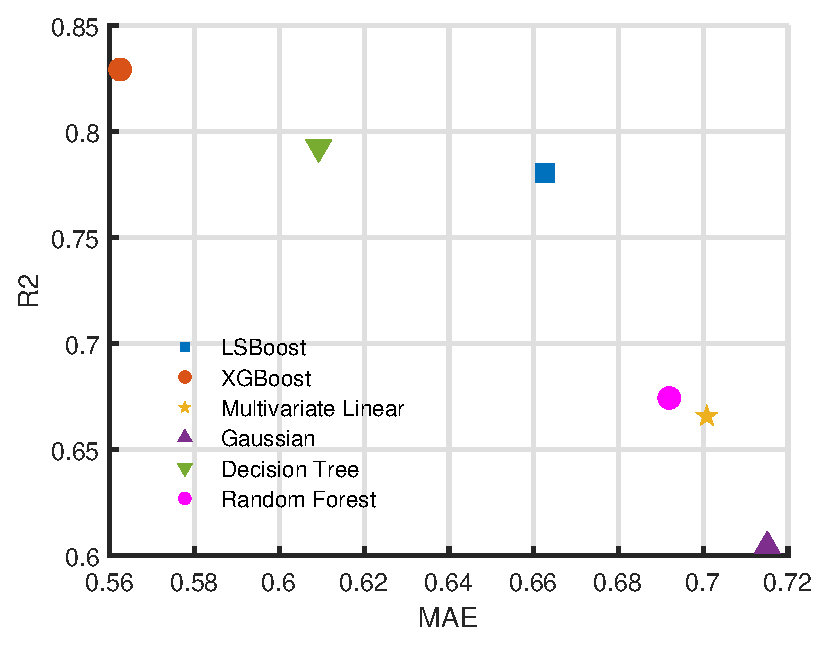
\includegraphics[width=\textwidth, keepaspectratio]{pics/multi-regression-compare-2.eps}
        % \caption{(d)} % Subfigure label
        % \label{fig:performance2}
    \end{minipage}
    
    \caption{Performance comparison of different regression models for predicting Tier 1 Gold medal prediction model. Subfigures illustrate different comparisons across models.}
    \label{fig:model_comparison}
\end{figure}


\subsection{Model Selection}

The best-performing model is selected using the TOPSIS (Technique for Order Preference by Similarity to Ideal Solution) method. This approach ensures a balanced evaluation by simultaneously considering models with:
\begin{itemize}
    \item Smaller values of MAE, MAPE, MSE, and RMSE.
    \item Larger values of $R^2$ (closer to 1 indicates better fit).
\end{itemize}

Among the Tier 1 Gold medal prediction models, for instance, XGBoost exhibited the best performance after evaluation.
It's also shown later in practice that each medal type can have very different best models.

\subsection{Model Optimization}

We apply various optimization algorithms to enhance model performance further. The algorithms tested include:
SSA \cite{8}, DBO \cite{9}, SCA \cite{10}, SA \cite{11}, PSO \cite{12}, SO \cite{13}, POA \cite{14},  
GWO \cite{15}.

As an example, SSA algorithm demonstrated the best results for optimizing the Tier 1 Gold medal prediction model, and the optimization outcome is shown in \textit{Figure~\ref{fig:smaller_eps_images}}.

\begin{figure}[htbp]
    \centering
    % First row
    \begin{minipage}[t]{0.3\textwidth}
        \centering
        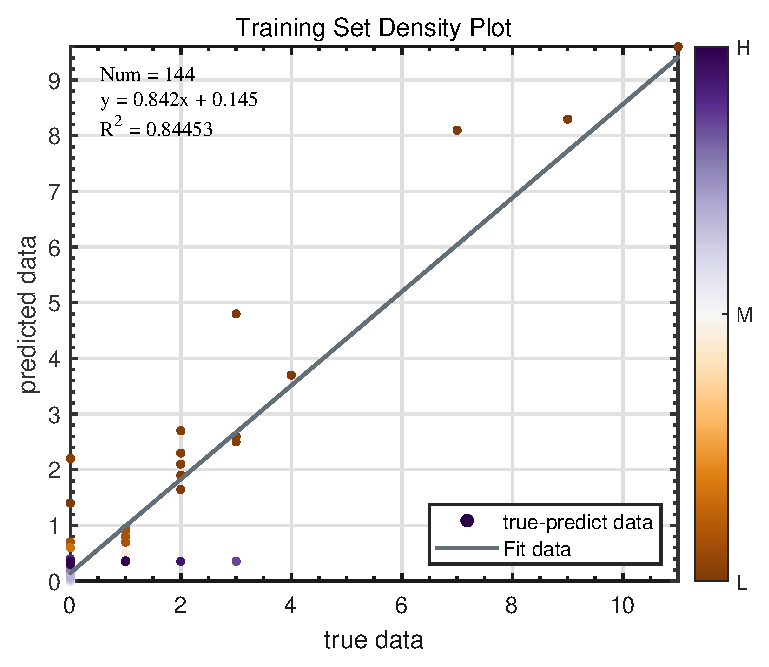
\includegraphics[width=2.2in, keepaspectratio]{pics/1.eps}
        \label{fig:image1}
    \end{minipage}
    \hfill
    \begin{minipage}[t]{0.3\textwidth}
        \centering
        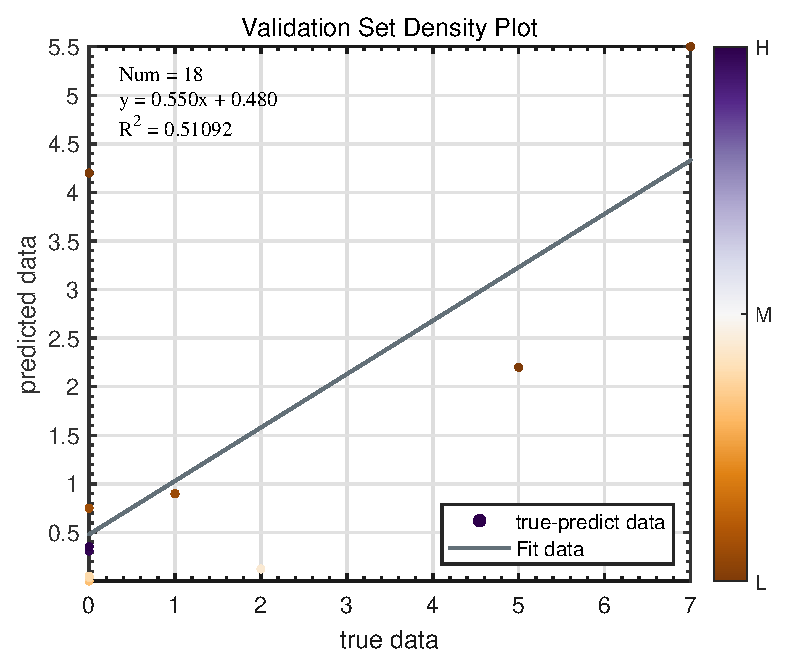
\includegraphics[width=2.2in, keepaspectratio]{pics/3.eps}
        \label{fig:image2}
    \end{minipage}
    \hfill
    \begin{minipage}[t]{0.3\textwidth}
        \centering
        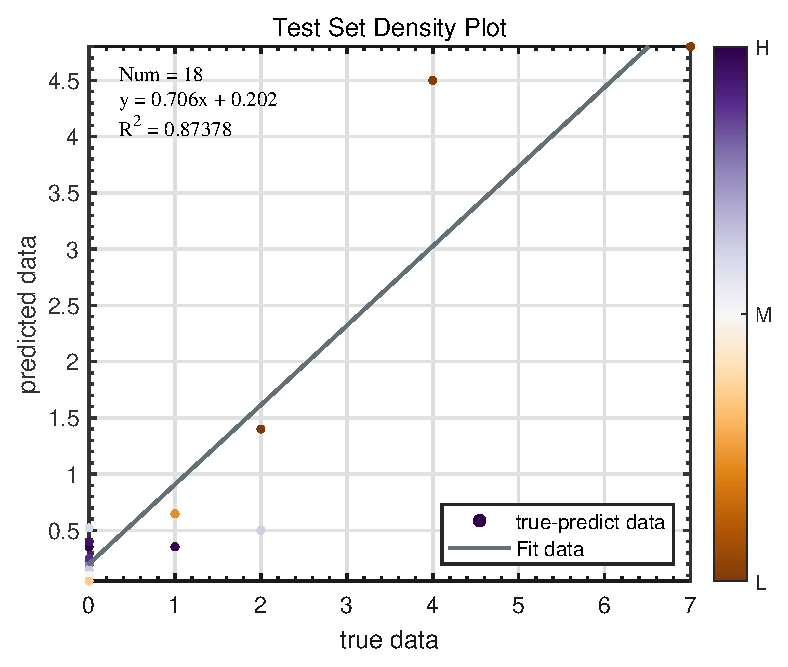
\includegraphics[width=2.2in, keepaspectratio]{pics/5.eps}
        \label{fig:image3}
    \end{minipage}
    
    \vspace{0.4cm} % Space between rows
    
    % Second row
    \begin{minipage}[t]{0.3\textwidth}
        \centering
        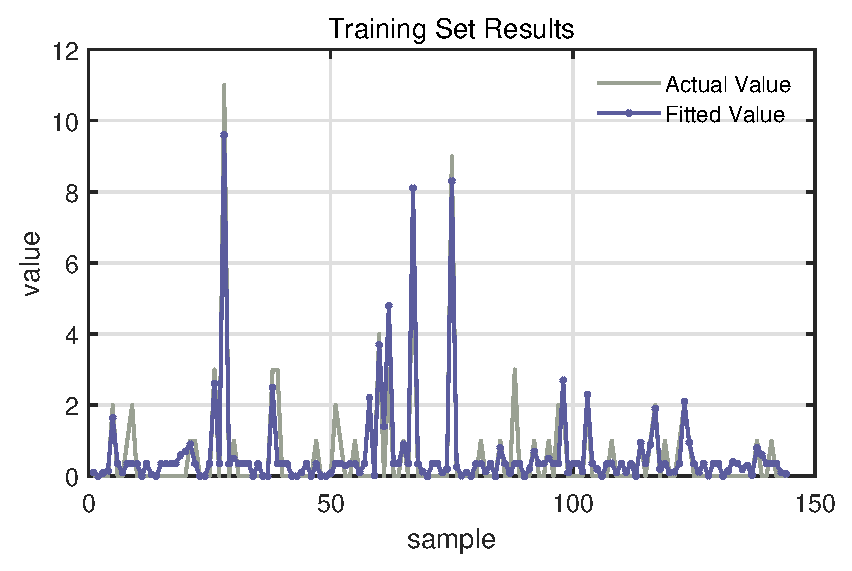
\includegraphics[width=2.2in, keepaspectratio]{pics/2.eps}
        \label{fig:image4}
    \end{minipage}
    \hfill
    \begin{minipage}[t]{0.3\textwidth}
        \centering
        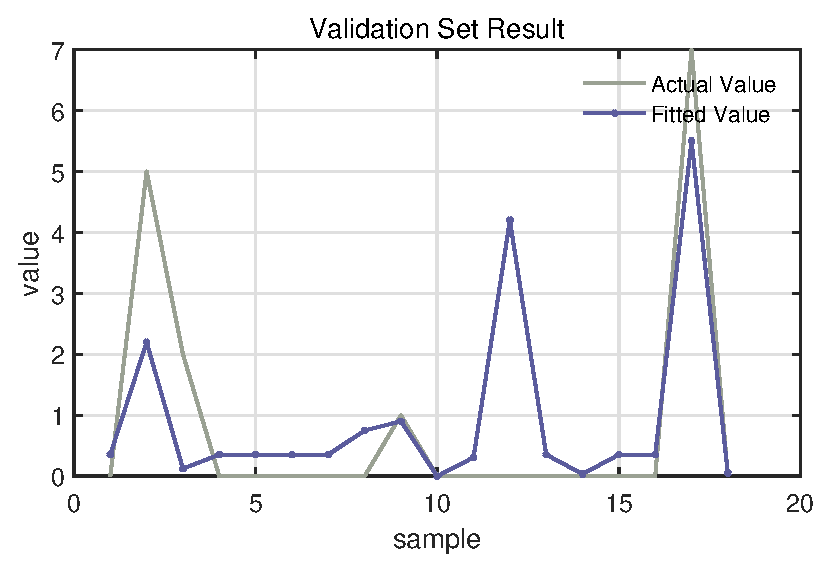
\includegraphics[width=2.2in, keepaspectratio]{pics/4.eps}
        \label{fig:image5}
    \end{minipage}
    \hfill
    \begin{minipage}[t]{0.3\textwidth}
        \centering
        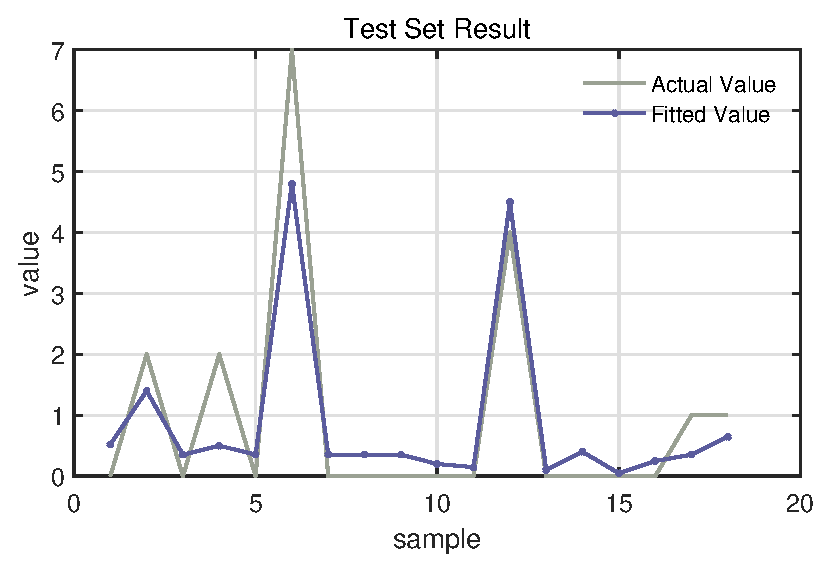
\includegraphics[width=2.2in, keepaspectratio]{pics/6.eps}
        \label{fig:image6}
    \end{minipage}
    
    \caption{Density plot and result of training set, validation set, and test set for Tier 1 Gold medal prediction model.}

    
    \label{fig:smaller_eps_images}
\end{figure}

\begin{wrapfigure}{r}{8cm}  %这是图文混排的环境
    \centering
    % 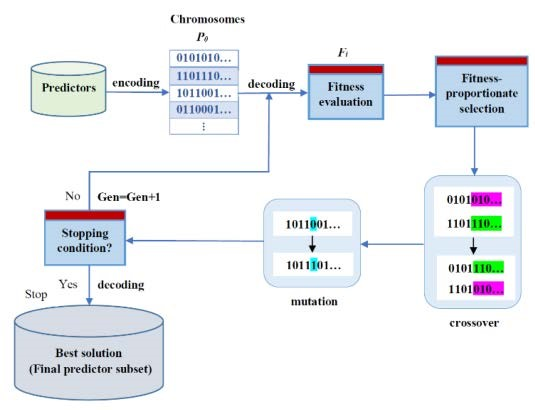
\includegraphics[width=0.9\linewidth,height=6cm]{pics/Multi-Agent_Optimization_Algorithm.jpg}
    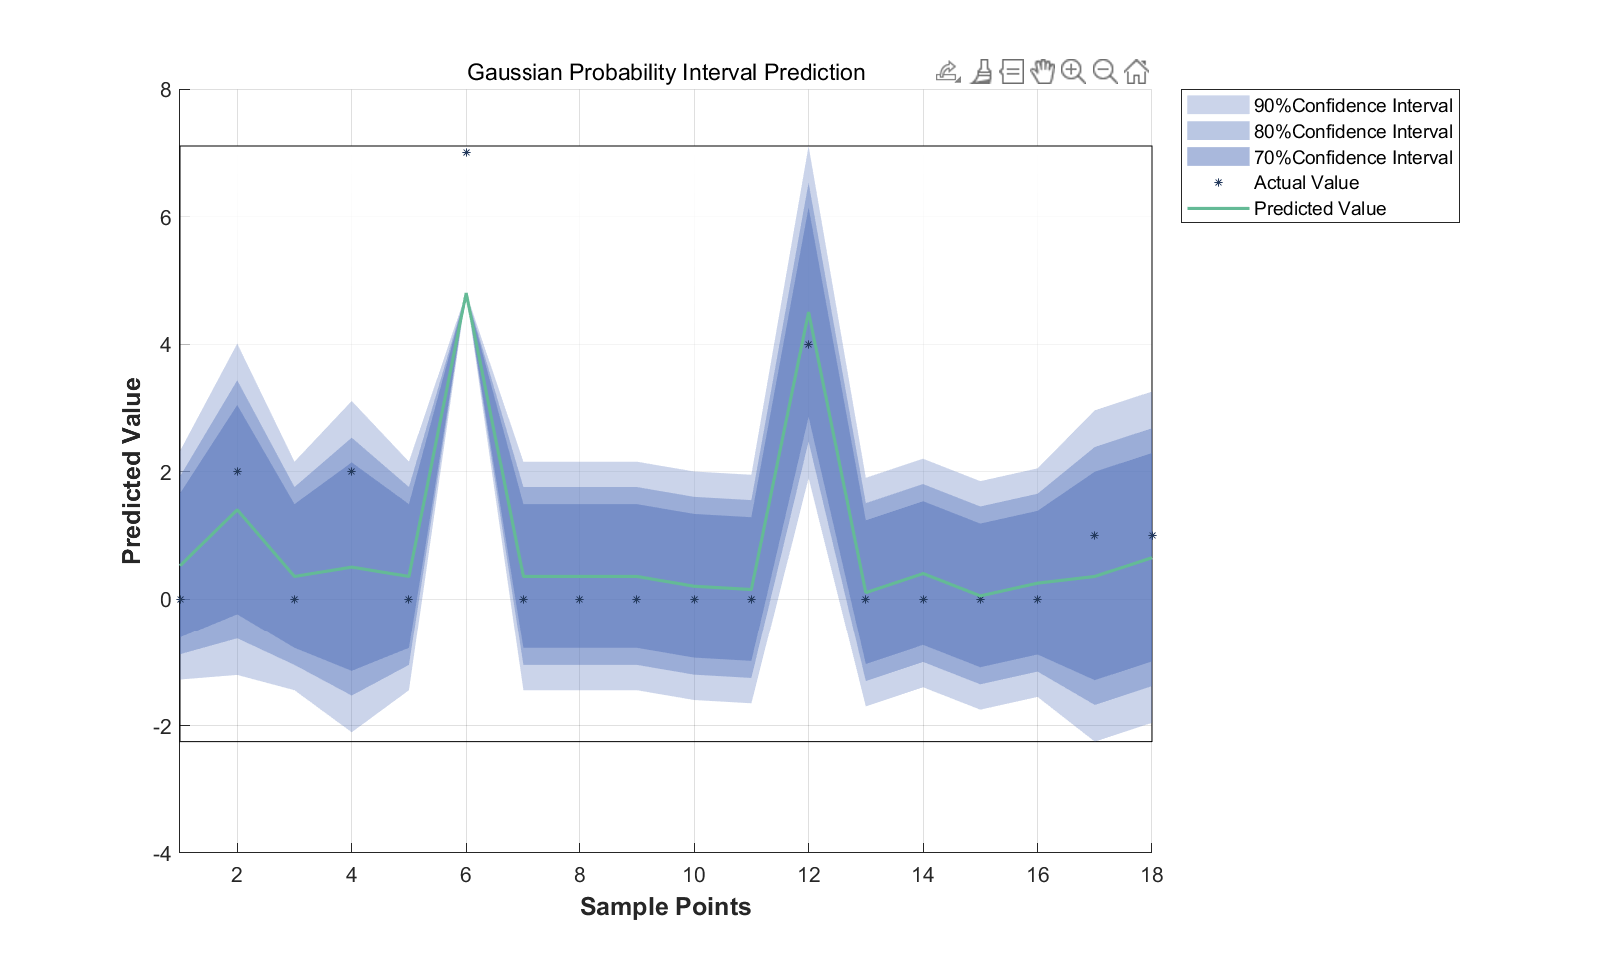
\includegraphics[width=0.5\textwidth]{pics/Gaussian Probability Interval Prediction.eps}
    \caption{Gaussian Probability Interval Prediction.}
    \label{fig:Probability_Interval_Prediction}
\end{wrapfigure}
\subsection{Uncertainty Quantification and Prediction Intervals}

To quantify the uncertainty in model predictions, we use Gaussian Probability Interval Prediction. This method calculates prediction intervals, providing upper and lower bounds for the estimated medal counts. The intervals represent the range within which the actual medal counts are expected to fall within at a specified confidence level, as shown in \textit{Figure~\ref{fig:Probability_Interval_Prediction}}.

\subsection{Conclusion}

The tier-based regression modeling approach provides a structured and efficient framework for predicting Olympic medal counts. By incorporating historical performance, host nation effects, and optimization techniques, the model achieves robust performance and reliable projections. The results offer actionable insights for countries aiming to improve their Olympic performance.

\section{Task1 --- Employing the model for prediction}

\subsection{Subtask 1 --- Predicting Medal Counts for the 2028 Los Angeles Olympics}

\subsubsection{Prediction Results}
We tested the established model to predict medal counts for the 2028 Los Angeles Olympics. The resulting medal table is presented as \textit{Table~\ref{tab:medal_counts}}: (results rounded to one decimal place, and the prediction intervals attached are calculated at a 95\% confidence level)

\begin{table}[htbp]
    \centering
    \begin{tabular}{|c|c|c|c|c|c|c|c|c|c|c|}
        \hline
        NOC & B & S & G & BL & BU & SL & SU & GL & GU & Tot \\
        \hline
        USA & 48.8 & 45.3 & 45.9 & 46.3 & 51.3 & 43.9 & 46.8 & 43.3 & 48.6 & 140.1 \\
        CHN & 27.3 & 30.1 & 46.7 & 25 & 29.6 & 28.8 & 31.4 & 44.3 & 49.1 & 104.1 \\
        GBR & 38.8 & 24.6 & 20.5 & 36.5 & 41.1 & 23.3 & 25.9 & 18.1 & 22.9 & 83.9 \\
        JPN & 19.1 & 22 & 26.3 & 16.8 & 21.4 & 20.7 & 23.3 & 23.9 & 28.7 & 67.4 \\
        FRA & 30.4 & 12.1 & 21.3 & 28.1 & 32.7 & 10.8 & 13.4 & 18.9 & 23.7 & 63.8 \\
        AUS & 18.3 & 15.4 & 21.7 & 16 & 20.6 & 14.1 & 16.7 & 19.3 & 24.1 & 55.4 \\
        ITA & 15.4 & 11.5 & 13.6 & 13.1 & 17.7 & 10.2 & 12.9 & 11.2 & 16 & 40.6 \\
        NED & 17 & 10.1 & 11.7 & 14.7 & 19.3 & 8.8 & 11.4 & 9.3 & 14.1 & 38.9 \\
        GER & 6.4 & 18 & 10.8 & 4.1 & 8.7 & 16.6 & 19.3 & 8.4 & 13.2 & 35.2 \\
        CAN & 11.5 & 5.5 & 10.5 & 9.2 & 13.7 & 4.2 & 6.8 & 8.1 & 12.9 & 27.4 \\
        KOR & 10.7 & 7.9 & 7.8 & 8.4 & 13 & 6.6 & 9.2 & 5.4 & 10.2 & 26.4 \\
        BRA & 5.6 & 8.2 & 6.8 & 3.3 & 7.9 & 6.9 & 9.5 & 4.4 & 9.2 & 20.6 \\
        NZL & 1.7 & 5.5 & 12.5 & 0 & 4 & 4.2 & 6.8 & 10.1 & 14.9 & 19.8 \\
        UKR & 7.9 & 5.2 & 5.7 & 5.6 & 10.2 & 3.9 & 6.5 & 3.3 & 8.1 & 18.8 \\
        ESP & 7.5 & 5.7 & 2.6 & 5.2 & 9.8 & 4.4 & 7 & 0.2 & 5 & 15.8 \\
        HUN & 3.9 & 7.5 & 3 & 1.6 & 6.2 & 6.2 & 8.8 & 0.6 & 5.4 & 14.3 \\
        AZE & 5 & 5.2 & 3 & 2.7 & 7.3 & 3.9 & 6.5 & 0.6 & 5.4 & 13.2 \\
        DEN & 6.6 & 3.8 & 2.3 & 4.3 & 8.9 & 2.5 & 5.1 & 0 & 4.8 & 12.7 \\
        BEL & 5.5 & 2 & 5.2 & 3.2 & 7.8 & 0.7 & 3.3 & 2.8 & 7.6 & 12.7 \\
        IRI & 4.9 & 3.1 & 3.5 & 2.6 & 7.2 & 1.8 & 4.4 & 1.1 & 5.9 & 11.5 \\
        JAM & 2.5 & 6.6 & 2.3 & 0.2 & 4.8 & 5.3 & 7.9 & 0 & 4.7 & 11.4 \\
        KAZ & 4.6 & 3.8 & 2.8 & 2.3 & 6.9 & 2.5 & 5.2 & 0.4 & 5.2 & 11.3 \\
        CUB & 5.7 & 3.2 & 2.1 & 3.4 & 8 & 1.9 & 4.5 & 0 & 4.5 & 11.1 \\
        KEN & 3.2 & 5.4 & 2.4 & 0.9 & 5.5 & 4 & 6.7 & 0 & 4.8 & 11 \\
        SWE & 3.2 & 3.6 & 3.9 & 0.9 & 5.5 & 2.3 & 4.9 & 1.5 & 6.3 & 10.7 \\
        SUI & 5.7 & 2.5 & 2.4 & 3.4 & 8 & 1.2 & 3.8 & 0 & 4.8 & 10.6 \\
        POL & 4.6 & 2.2 & 3.2 & 2.3 & 6.9 & 0.9 & 3.5 & 0.8 & 5.6 & 9.9 \\
        GRE & 6.8 & 1.2 & 0.7 & 4.5 & 9.1 & 0 & 2.6 & 0 & 3.1 & 8.7 \\
        UZB & 3.2 & 3.1 & 2.4 & 0.9 & 5.5 & 1.8 & 4.4 & 0 & 4.8 & 8.7 \\
        GEO & 3.2 & 2.4 & 2.7 & 0.9 & 5.5 & 1.1 & 3.8 & 0.3 & 5.1 & 8.4 \\
        LTU & 3.2 & 1.6 & 2.5 & 0.9 & 5.5 & 0.3 & 2.9 & 0.1 & 4.9 & 7.3 \\
        CRO & 3.1 & 3.2 & 0.9 & 0.8 & 5.4 & 1.9 & 4.5 & 0 & 3.3 & 7.3 \\
        TUR & 4.8 & 2.6 & 0 & 2.5 & 7.1 & 1.3 & 3.9 & 0 & 2.1 & 7.1 \\
        ROU & 3.3 & 0.9 & 2.9 & 1 & 5.6 & 0 & 2.2 & 0.5 & 5.3 & 7.1 \\
        BUL & 2.5 & 1.4 & 3 & 0.2 & 4.8 & 0.1 & 2.7 & 0.6 & 5.4 & 6.9 \\
        NOR & 3.8 & 1.4 & 1.4 & 1.5 & 6.1 & 0.1 & 2.7 & 0 & 3.8 & 6.6 \\
        THA & 2.6 & 2.3 & 1.5 & 0.3 & 4.9 & 1 & 3.6 & 0 & 3.9 & 6.4 \\
        CZE & 2 & 2.7 & 1.4 & 0 & 4.2 & 1.4 & 4.1 & 0 & 3.8 & 6.1 \\
        RSA & 2.1 & 3.4 & 0.6 & 0 & 4.4 & 2 & 4.7 & 0 & 3 & 6.1 \\
        ETH & 1 & 2.8 & 1.2 & 0 & 3.3 & 1.5 & 4.1 & 0 & 3.6 & 5 \\
        TPE & 2.2 & 1.3 & 1.5 & 0 & 4.5 & 0 & 2.6 & 0 & 3.9 & 5 \\
        IND & 1.4 & 1.9 & 1.6 & 0 & 3.7 & 0.5 & 3.2 & 0 & 4 & 4.9 \\
        MEX & 2.2 & 2.7 & 0 & 0 & 4.5 & 1.4 & 4 & 0 & 2.2 & 4.8 \\
        ... & ... & ... & ... & ... & ... & ... & ... & ... & ... & ... \\
    \end{tabular}
    \caption{Predicted medal counts for 2028 Los Angeles Olympics. B: Bronze, S: Silver, G: Gold, BL: Bronze Lower Bound, BU: Bronze Upper Bound, SL: Silver Lower Bound, SU: Silver Upper Bound, GL: Gold Lower Bound, GU: Gold Upper Bound. Due to space constraints, only the top 43 countries are shown.}
    \label{tab:medal_counts}
\end{table}

\subsubsection{Analysis of Prediction Results}

In this section, we analyze the improvements or declines in medal counts. We define \textit{"improvement"} and \textit{"decline"} as follows in order to separate them from normal fluctuations:

\begin{itemize}
    \item \textbf{Improvement:} If the predicted medal count for a country in 2028 is higher than its medal count from the previous Olympics more than a constant \textit{X} percent (\textbf{Condition 1}) or for every type of medal, the count doesn't decrease and at least one type of medal shows an increase in count (\textbf{Condition 2}), we consider it an improvement.
    \item \textbf{Decline:} If the predicted medal count for a country in 2028 is lower than its medal count from the previous Olympics more than a constant \textit{X} percent (\textbf{Condition 1}) or for every type of medal, the count doesn't increase and at least one type of medal shows a decrease in count (\textbf{Condition 2}), we consider it a decline.
\end{itemize}

With \textit{X} set to 15\%, we identified the following countries that are expected to improve or decline in medal counts at the 2028 Los Angeles Olympics shown in \textit{Table~\ref{tab:medal_changes}}.

\begin{table}[htbp]
    \centering
    \begin{tabular}{|c|c|c||c|c|c|}
        \hline
        NOC & Change & Conditions Met & NOC & Change & Conditions Met \\
        \hline
        ARG & $\uparrow$ & 1, 2 & KAZ & $\uparrow$ & 1, 2 \\
        AZE & $\uparrow$ & 1, 2 & SUI & $\uparrow$ & 1, 2 \\
        BEL & $\uparrow$ & 1 & SVK & $\uparrow$ & 1 \\
        CHN & $\uparrow$ & 2 & UKR & $\uparrow$ & 1, 2 \\
        CUB & $\uparrow$ & 1 & USA & $\uparrow$ & 2 \\
        DEN & $\uparrow$ & 1, 2 & HUN & $\downarrow$ & 1 \\
        ETH & $\uparrow$ & 1 & IND & $\downarrow$ & 1 \\
        GBR & $\uparrow$ & 1, 2 & KOR & $\downarrow$ & 1 \\
        GEO & $\uparrow$ & 1 & MAR & $\downarrow$ & 1 \\
        INA & $\uparrow$ & 1 & NOR & $\downarrow$ & 1 \\
        JAM & $\uparrow$ & 1, 2 & POR & $\downarrow$ & 1 \\
        JPN & $\uparrow$ & 1, 2 & ROU & $\downarrow$ & 1 \\
        \hline
    \end{tabular}
    \caption{Countries with Predicted Changes in Medal Counts for the 2028 Los Angeles Olympics}
    \label{tab:medal_changes}
\end{table}

\subsection{Subtask 2 --- Predicting the Number of Countries Winning Their First Medal}

In this subtask, we aim to predict the number of countries that will win their first Olympic medal at the 2028 Los Angeles Olympics. This involves analyzing historical data to identify trends and factors that contribute to countries winning their first medals and applying these insights to make predictions for the upcoming Olympics.

\subsubsection{Analysis}
Firstly, we calculated historical data on countries that have won their first Olympic medals in past Games, which is done in Data Preprocessing. The visualization of this dataset is shown in \textit{Figure~\ref{fig:cumulative_medal_winning_countries}} \AIcite{AI1}.

\begin{figure}[htbp]
    \centering
    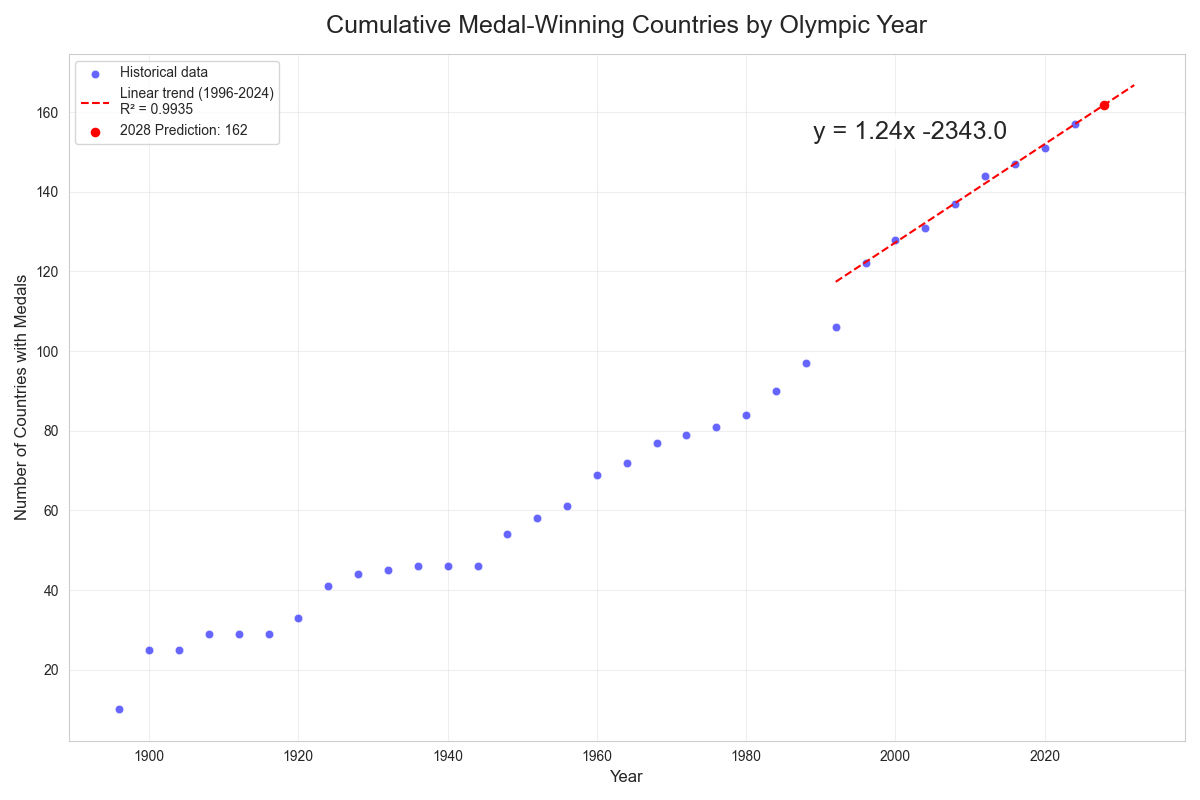
\includegraphics[width=0.8\textwidth]{pics/Cumulative Medal-Winning Countries by Olympic Year.png}
    \caption{Cumulative Medal-Winning Countries by Olympic Year}
    \label{fig:cumulative_medal_winning_countries}
\end{figure}


Looking at this figure we discovered that the data points of recent Olympics exhibit a strong linear relationship. Therefore, we applied linear regression to the data point of recent 8 Olympics (y represents the number of countries that have won their first Olympic medals in past Games, x represents year), the result was as follows.

\subsubsection{Validation}
\begin{Theorem}
    The confidence interval for the regression function $\mu (x_0)=\hat{a}x_0+\hat{b}$ at a confidence level of $(1-\alpha)$ is
    $$\bigg( \hat{a}x_0+\hat{b} \pm t_{\alpha /2,n-2}\cdot \sigma \sqrt{\frac{1}{n}+\frac{(x_0-\bar{x})^2}{S_{xx}}} \bigg)$$
\end{Theorem}

It's notable that $R^2=0.9935$, indicating a very high fit to the data, meaning the linear model is highly accurate for this dataset.

Then the projection for number of countries that have won medals till 2028 (x=2028) 
$\hat{y}_{2028}=\hat{a}x+\hat{b}=161.86$.
Therefore, the projection for new medal-winning countries in the next Olympics is
$\Delta y=\hat{y}_{2028}-y_{2024}=4.86$.


Based on our calculations, the residual standard deviation $\sigma = 0.917$, and $S_{xx} = \sum_{k=1}^{8}(x_k - \bar{x})^2 = 672$. For a 70\% confidence level, we refer to the t-distribution table and find $t_{0.15,6} = 1.134$.

\subsubsection{Results}

Based on our analysis and model predictions, we estimate that approximately \textbf{5} countries will win their first Olympic medal at the 2028 Los Angeles Olympics. This prediction is derived from the linear regression analysis of historical data, which shows a strong correlation ($R^2 = 0.9935$) between the year and the cumulative number of countries winning their first medal. The confidence interval for this prediction, at a 70\% confidence level, is between 4.05 and 5.67 new medal-winning countries.


\subsection{Subtask 3.1 --- Exploring the Relationship Between Event Count and Medal Count}

In this subtask, we investigate the relationship between the number and types of events a country participates in and the number of medals it earns. The analysis is performed using data from the 2024 Olympics, focusing on three primary aspects: visualization, correlation analysis, and interpretation of results.

\subsubsection{Visualization}
To better understand the relationship between event count and medal count, we employed two visualization methods:
\begin{itemize}
    \item \textbf{Scatter Plot}: Displays the relationship between event count and medal count.
    \item \textbf{Box Plot}: Analyzes the distribution of medal counts across different event count intervals.
\end{itemize}

    
\begin{figure}[!h]
    \begin{minipage}[t]{0.5\textwidth}
        \centering
        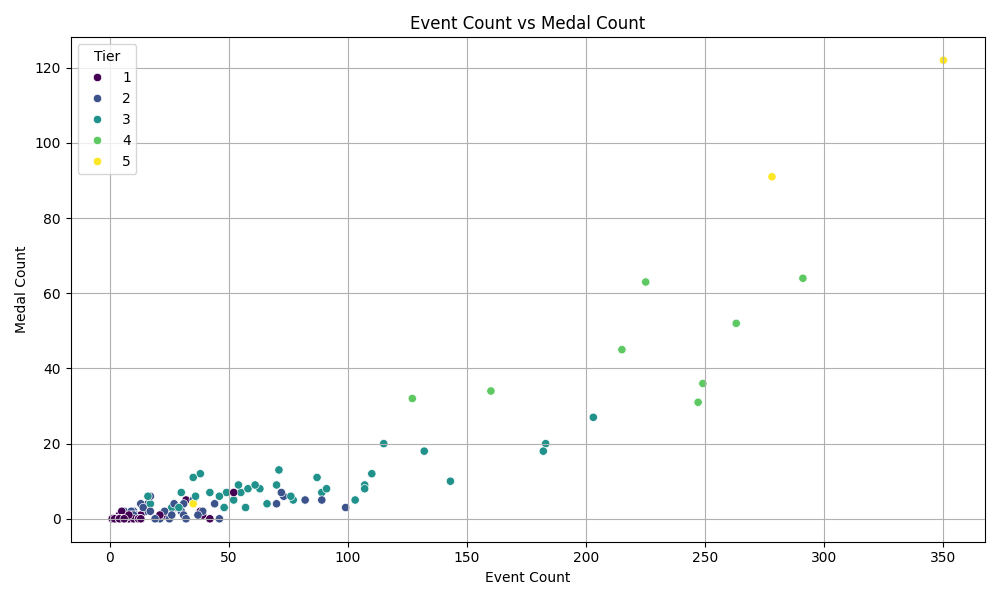
\includegraphics[width=1\textwidth]{pics/event_count_vs_medal_count.png}
    \end{minipage}
    \begin{minipage}[t]{0.5\textwidth}
        \centering
        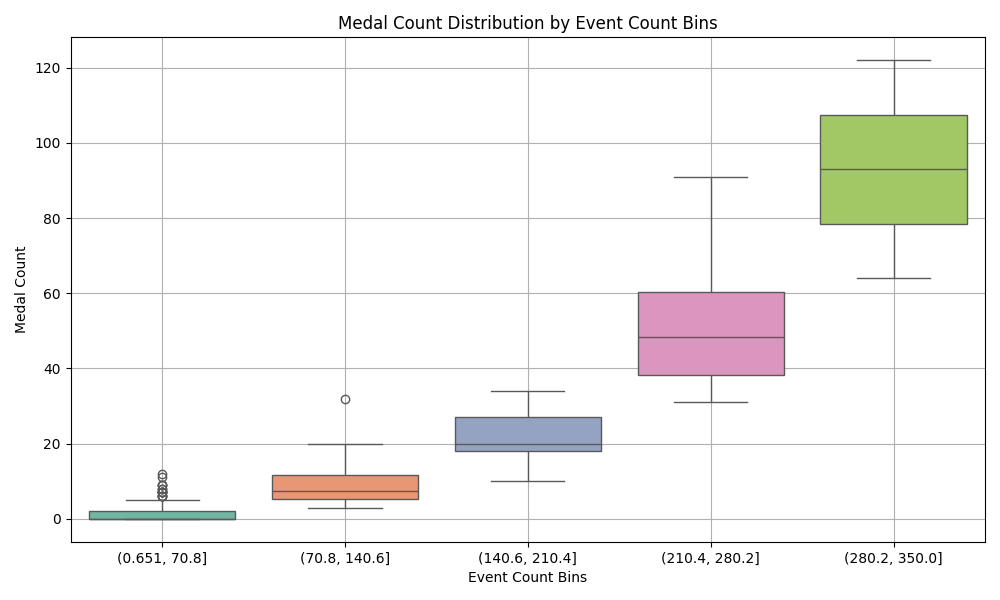
\includegraphics[width=1\textwidth]{pics/medal_count_distribution_by_event_count_bins.png}
    \end{minipage}
    \caption{Visualizations: (Left) Scatter plot showing the correlation; 
    (Right) Box plot depicting the distributions.}
\end{figure}

    To better understand the relationship between event count and medal count, countries were grouped into five distinct tiers based on their competitive performance using the K-means clustering algorithm. 

    The decision to use K-means clustering was motivated by the scatter plot observations, which suggested heterogeneous patterns in the event count and medal count relationship across different types of countries. The clustering process was informed by previous medal achievements(first gold medals, then total medals), ensuring that the grouping reflected meaningful competitive distinctions.
    
    %! TODO: Add the clustering result figure here
    
    
    Once the countries were assigned to tiers, we conducted separate correlation analyses within each tier. Spearman's correlation coefficient was used to measure the strength and direction of the relationship, as it is well-suited for non-parametric data and can handle potential non-linearity. The results are shown in following Table~\ref{tab1}.


%     \begin{wrapfigure}{r}{8cm}  %这是图文混排的环境
%         \centering
%         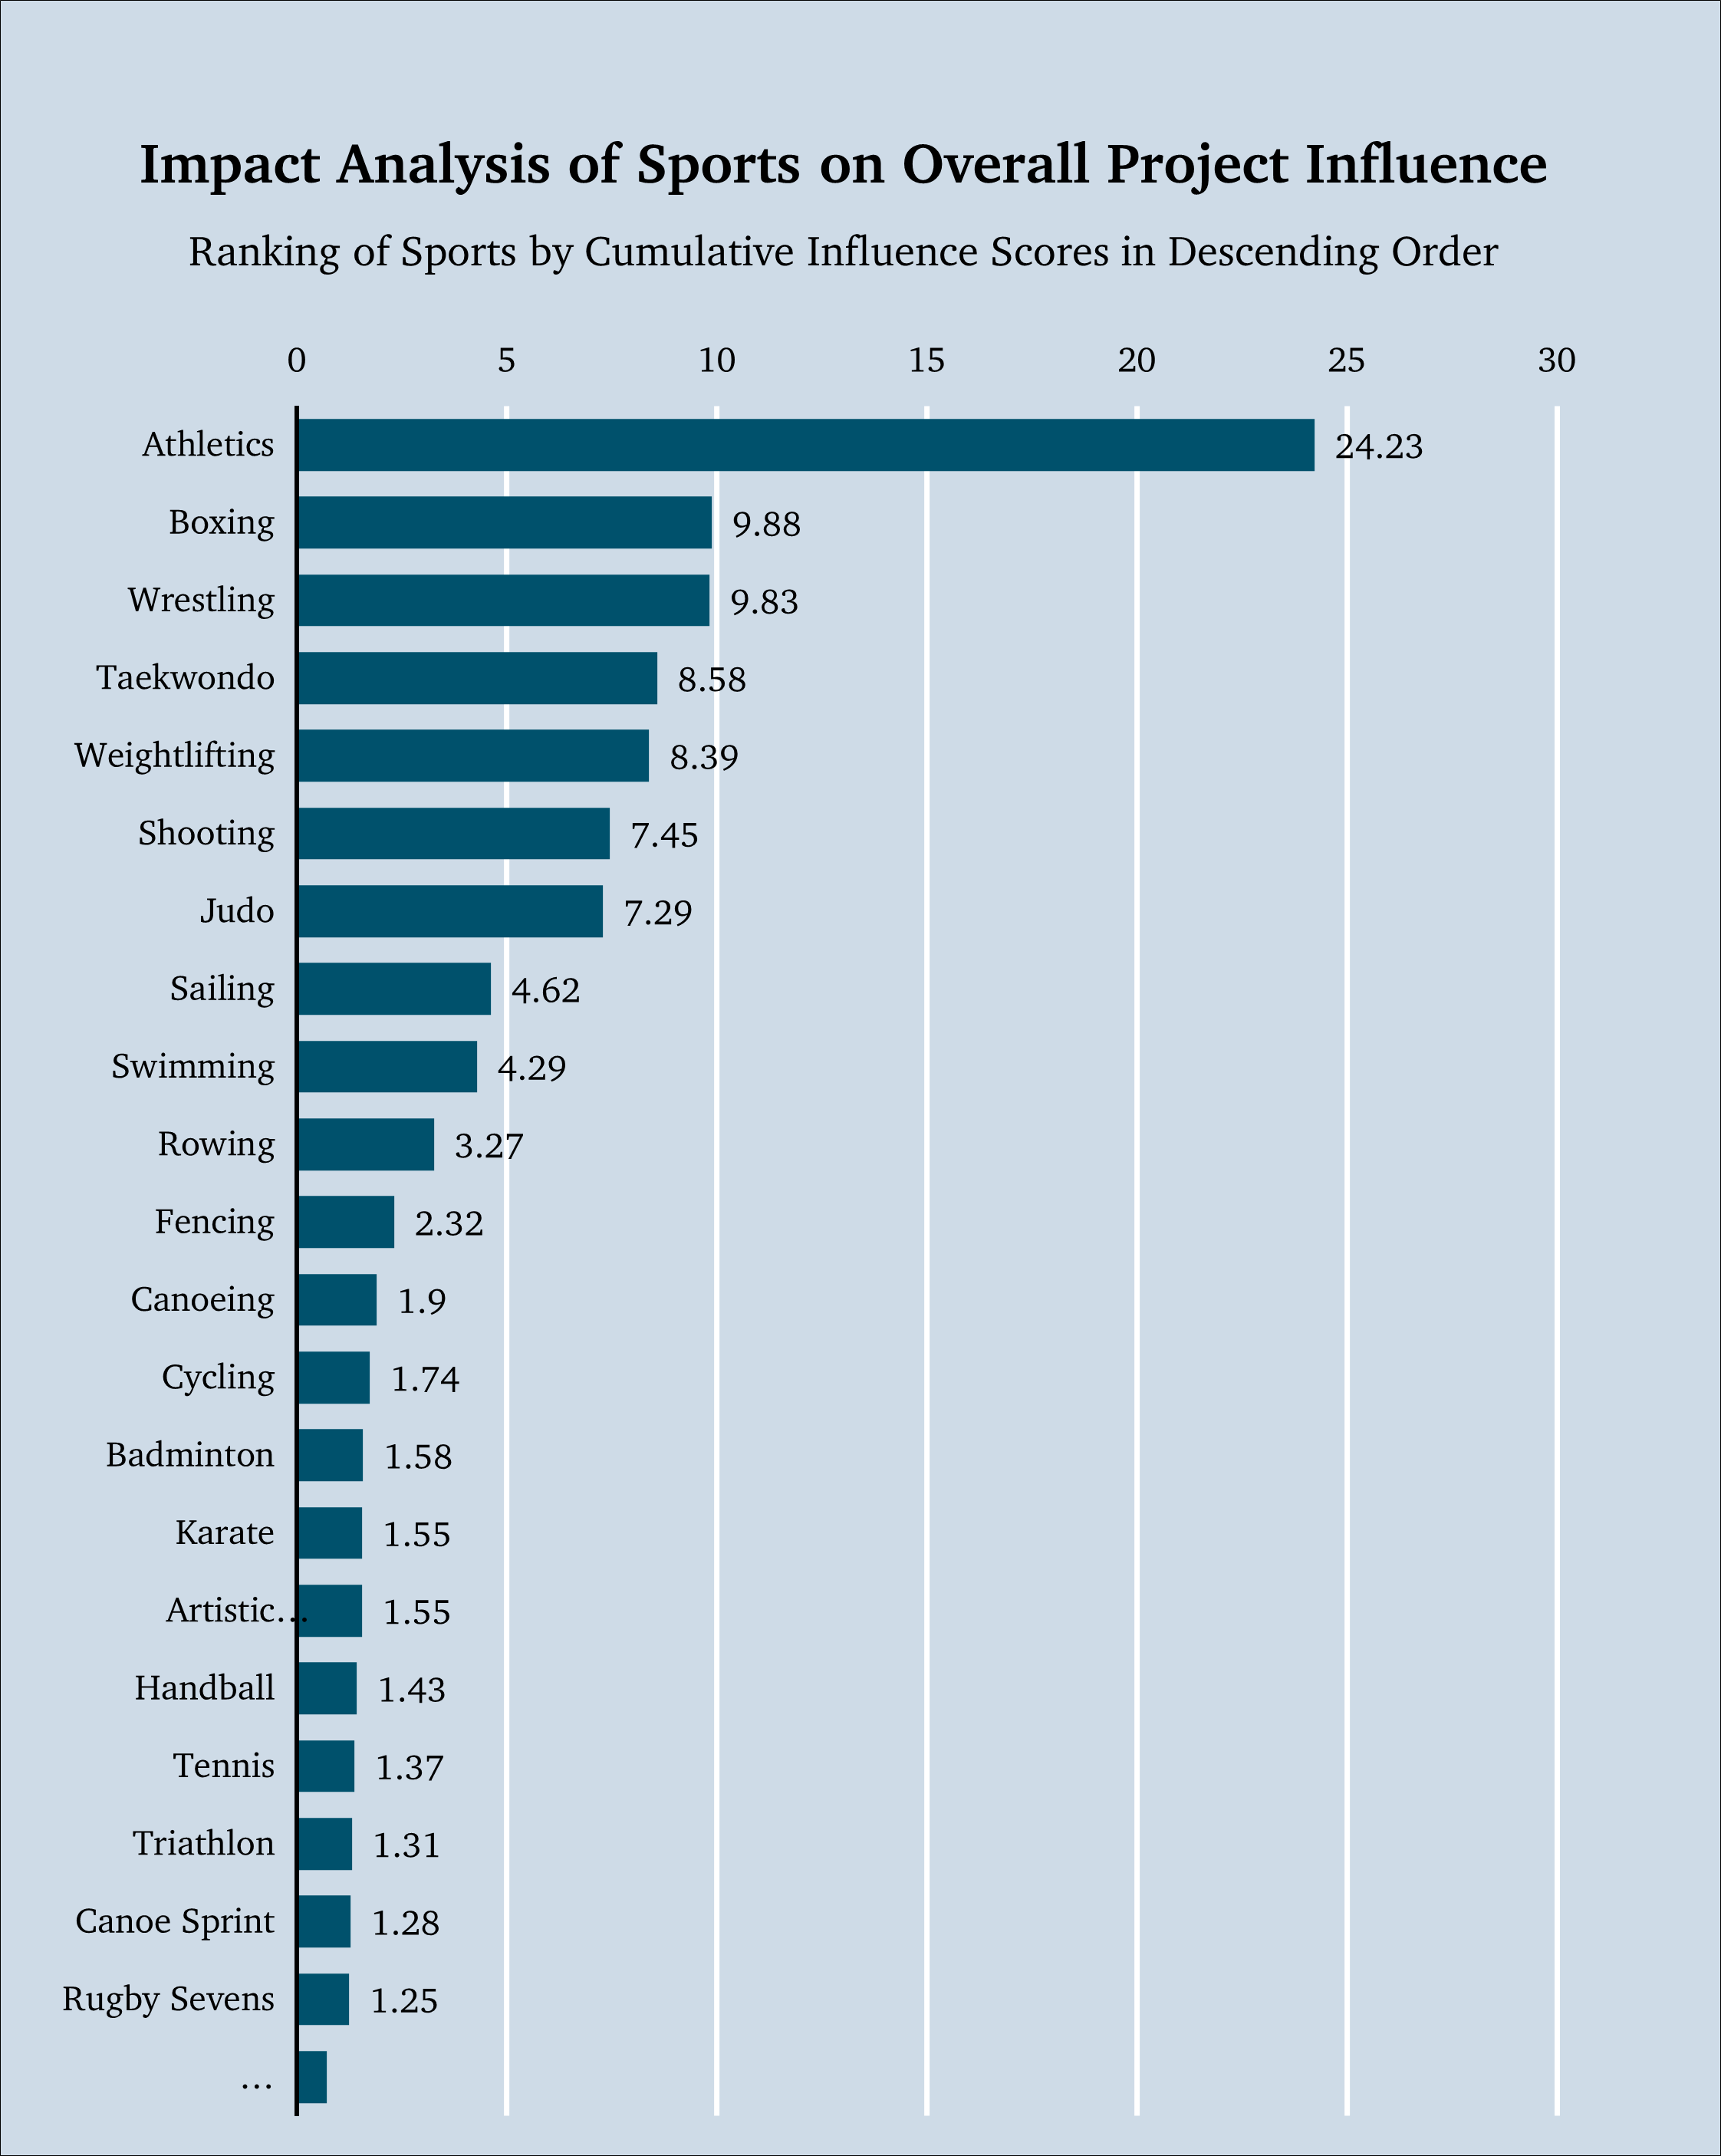
\includegraphics[width=0.9\linewidth,height=9cm]{pics/sport_influence_whole.png}
%         \caption{Ranking of sports by global importance based on aggregated event importance values across all countries.}
%         \label{fig:sport_importance}
%     \end{wrapfigure}
% \begin{table}[h!]
%     \centering
%     \begin{tabular}{ccc}
%     \toprule
%     \textbf{Tier} & \textbf{Spearman Correlation} & \textbf{p-value} \\

%     1 & 0.38 & $2.16 \times 10^{-5}$ \\
%     2 & 0.39 & $0.01$ \\
%     3 & 0.61 & $4.99 \times 10^{-5}$ \\
%     4 & 0.57 & $0.13$ \\
%     5 & 0.98 & $0.02$ \\
%     \bottomrule
%     \end{tabular}
%     \caption{Spearman correlation and p-values across different tiers.}
%     \label{tab1}
% \end{table}

\begin{wraptable}{r}{8cm}  %这是图文混排的环境
    \centering
    \begin{tabular}{ccc}
    \toprule
    \textbf{Tier} & \textbf{Spearman Correlation} & \textbf{p-value} \\ 
    \midrule
    1 & 0.38 & $2.16 \times 10^{-5}$ \\ 
    2 & 0.39 & $0.01$ \\ 
    3 & 0.61 & $4.99 \times 10^{-5}$ \\ 
    4 & 0.57 & $0.13$ \\ 
    5 & 0.98 & $0.02$ \\ 
    \bottomrule
    \end{tabular}
    \caption{Table \thetable: Spearman correlation and p-values across different tiers.}
    \label{tab1}
\end{wraptable}

\subsubsection{Interpretation of Results}
The analysis indicates that for most tiers (1, 2, 4, and 5), there is a statistically significant positive relationship between event count and medal count ($p < 0.05$). This suggests that the number of events a country participates in positively impacts its medal count. For Tier 3, the $p$-value is greater than 0.05, indicating no statistically significant correlation between event count and medal count within this group. This anomaly could be due to specific factors such as high variability in event outcomes or unmeasured country-specific attributes. However, the overall analysis aligns with the expectation that more competitive countries (higher tiers) are better equipped to convert event participation into medals due to superior resources, training, and athletes.

% \subsubsection{Conclusions and Recommendations(Optional)}
% \begin{itemize}
%     \item \textbf{Strategic Participation}: Select events with competitive advantage.
%     \item \textbf{Investment in Training and Resources}: Invest in infrastructure, coaching, and athlete preparation.
%     \item \textbf{Focus on Key Events}: Optimize performance in key events and expand into new events.
% \end{itemize}


\subsection{Subtask 3.2 --- Identifying the Most Important Sports for Various Countries}

% This subtask aims to determine the most significant sports for different countries based on their historical performance in the Olympics. To achieve this, we develop a method to calculate the importance of each event and sport, both at the country level and globally. 


\subsubsection{Methodology}
To answer the question of which sports are most important for various countries, we proceed with the following steps:

\paragraph{Step 1}

Compute the event importance value $w_{i,j} = \frac{m_{i,j}}{M_i}$, ensuring that the sum of importance values for all events for a given country satisfies $\sum_{j=1}^M w_{i,j} = 1$.

\paragraph{Step 2}
For each event $E_j$, we calculate its global importance value $W_j = \sum_{i=1}^N w_{i,j}$ as the sum of its importance values across all countries, which captures the relative importance of the event across all countries, regardless of individual country performance.

\paragraph{Step 3}
For each sport $S_k$, we compute its global importance $I_k = \sum_{j \in S_k} W_j$.It is completed through aggregating the global importance values $W_j$ of all events $E_j$ under the sport, providing an overall measure of the importance of each sport for all countries collectively.

\paragraph{Step 4}
The sports are then ranked based on their global importance values $I_k$. A visualization of the rankings illustrates that athletics, boxing, and wrestling are the top three most important sports globally, where athletics has the absolute highest(more than twice of the second place) importance value. Result is shown in \textit{Figure~\ref{fig:sport_importance}}.

\newpage

\begin{wrapfigure}{r}{8cm}  %这是图文混排的环境
    \centering
    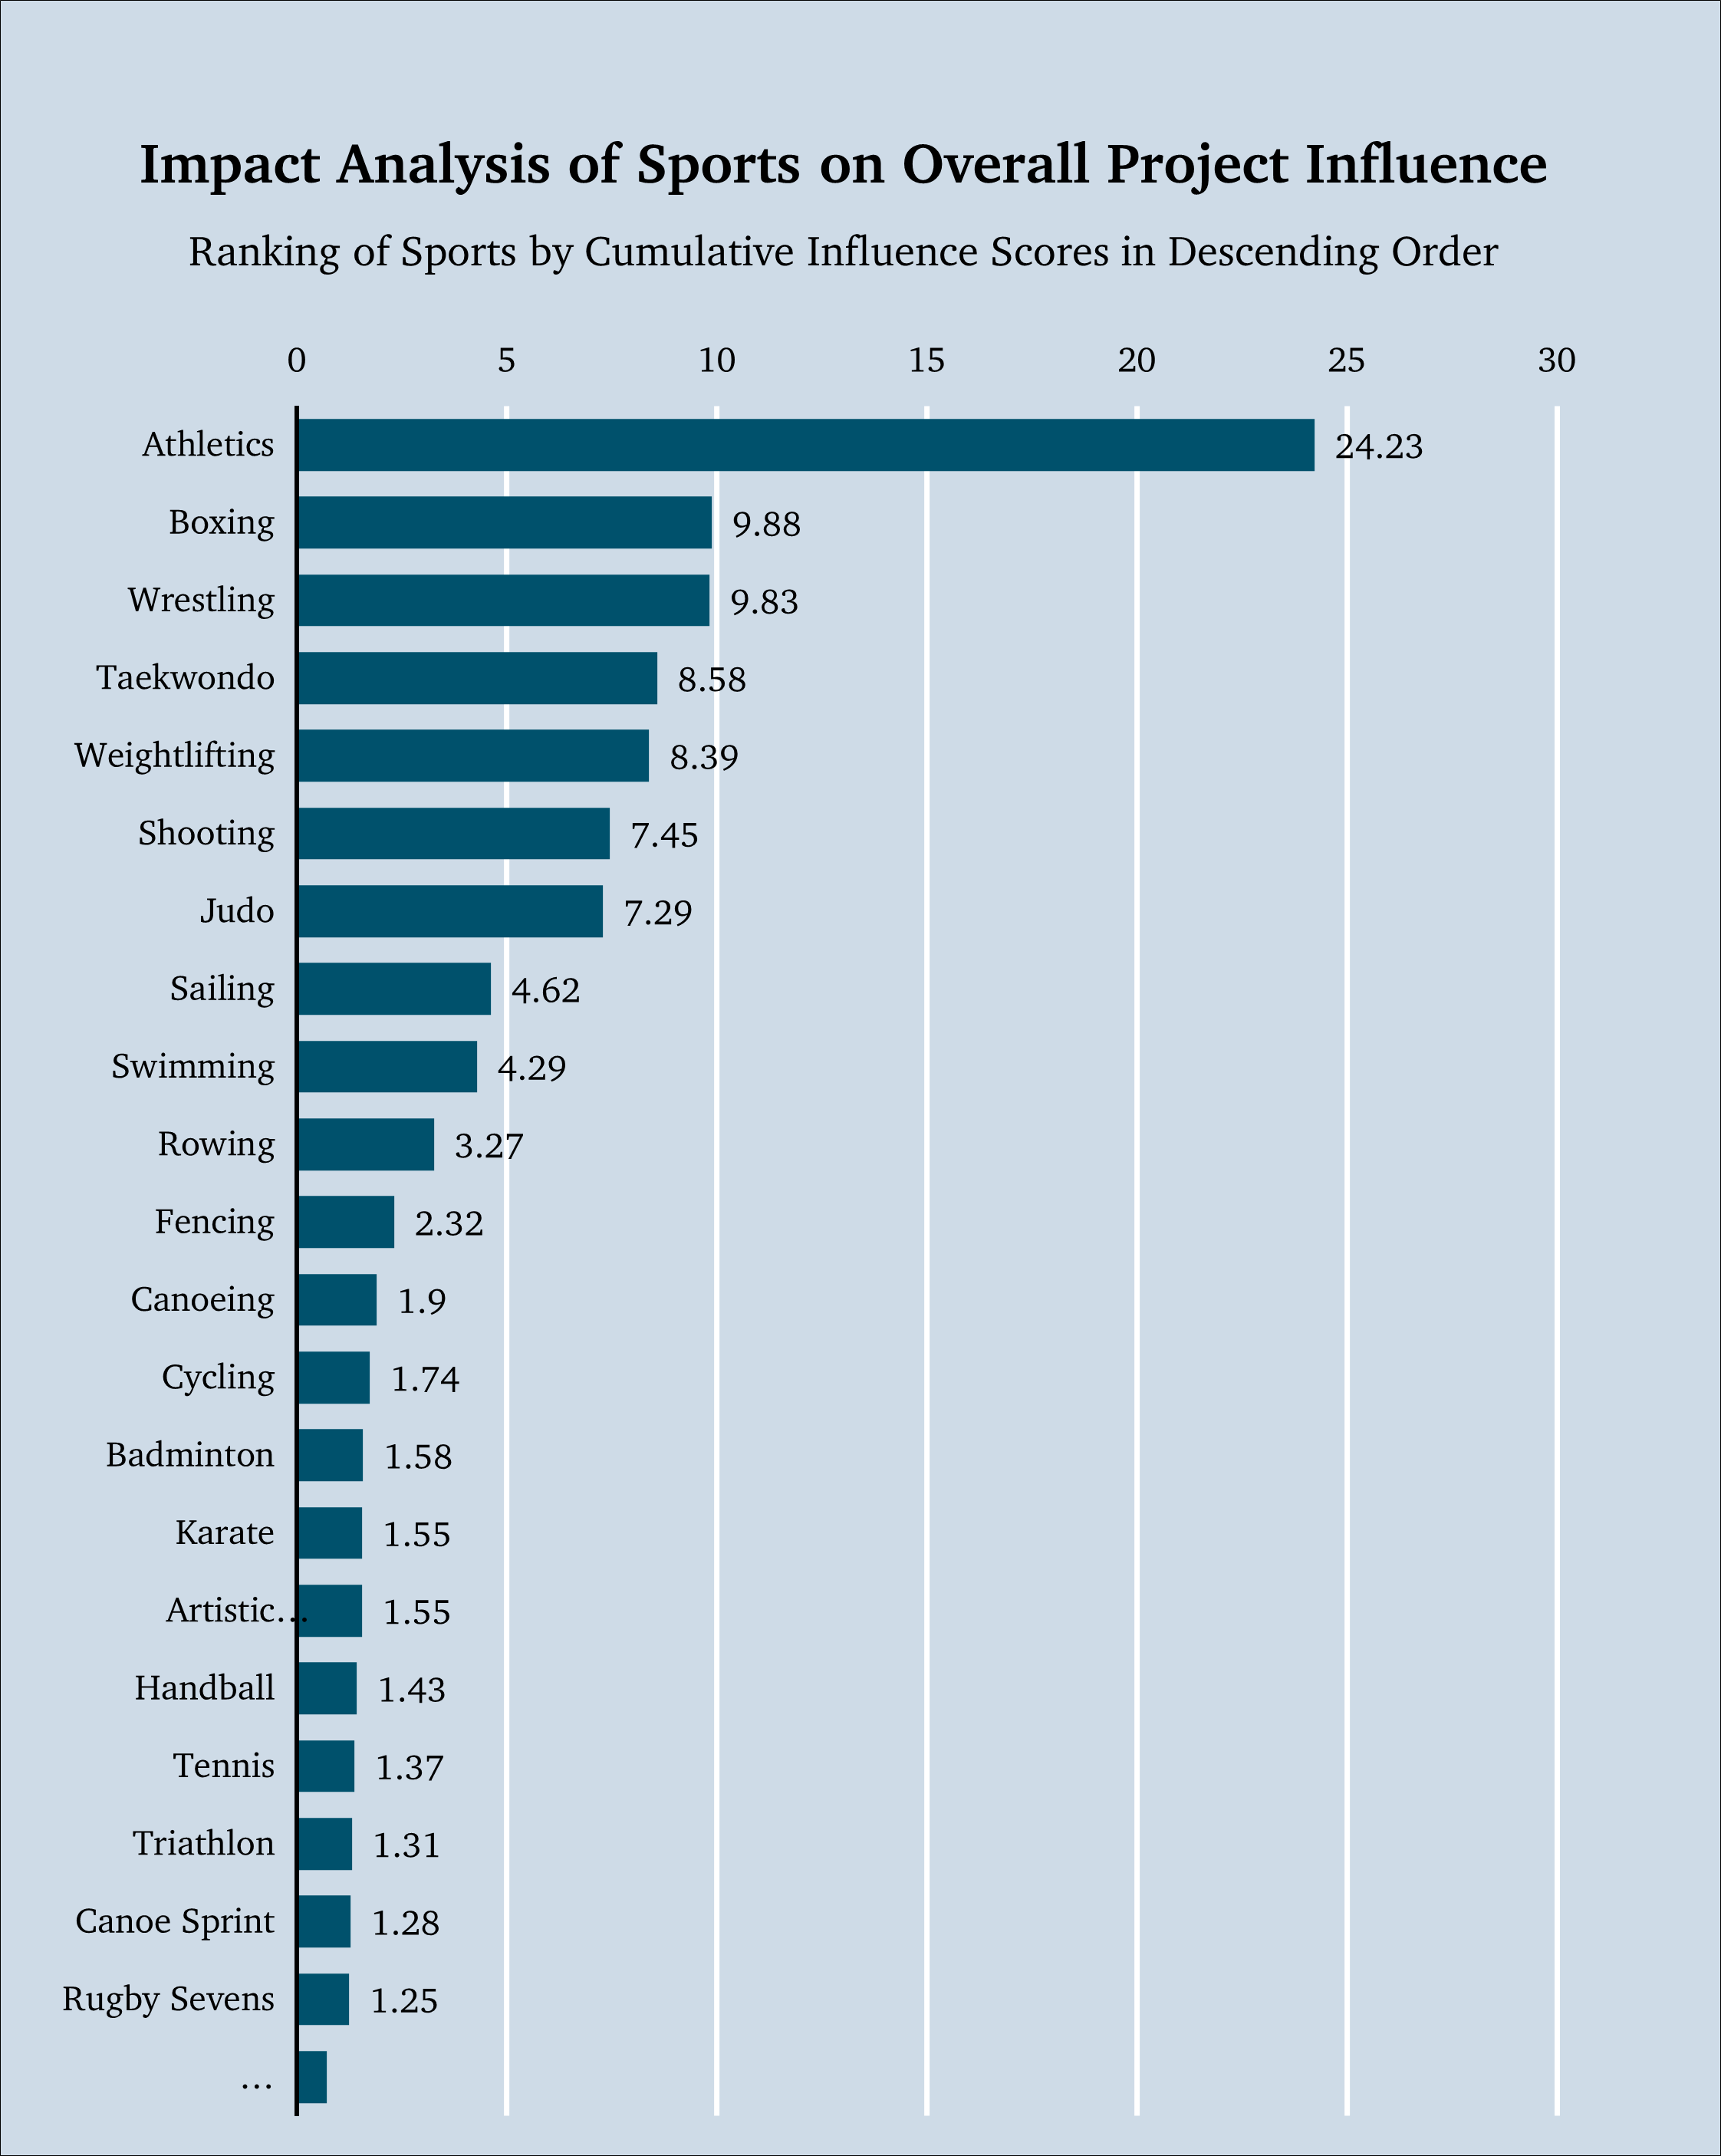
\includegraphics[width=0.9\linewidth,height=9cm]{pics/sport_influence_whole.png}
    \caption{Ranking of sports by global importance based on aggregated event importance values across all countries.}
    \label{fig:sport_importance}
\end{wrapfigure}
% \newpage
% \begin{wrapfigure}[12]{r}{0.5\textwidth} % Adjusted height and width
%     \centering
%     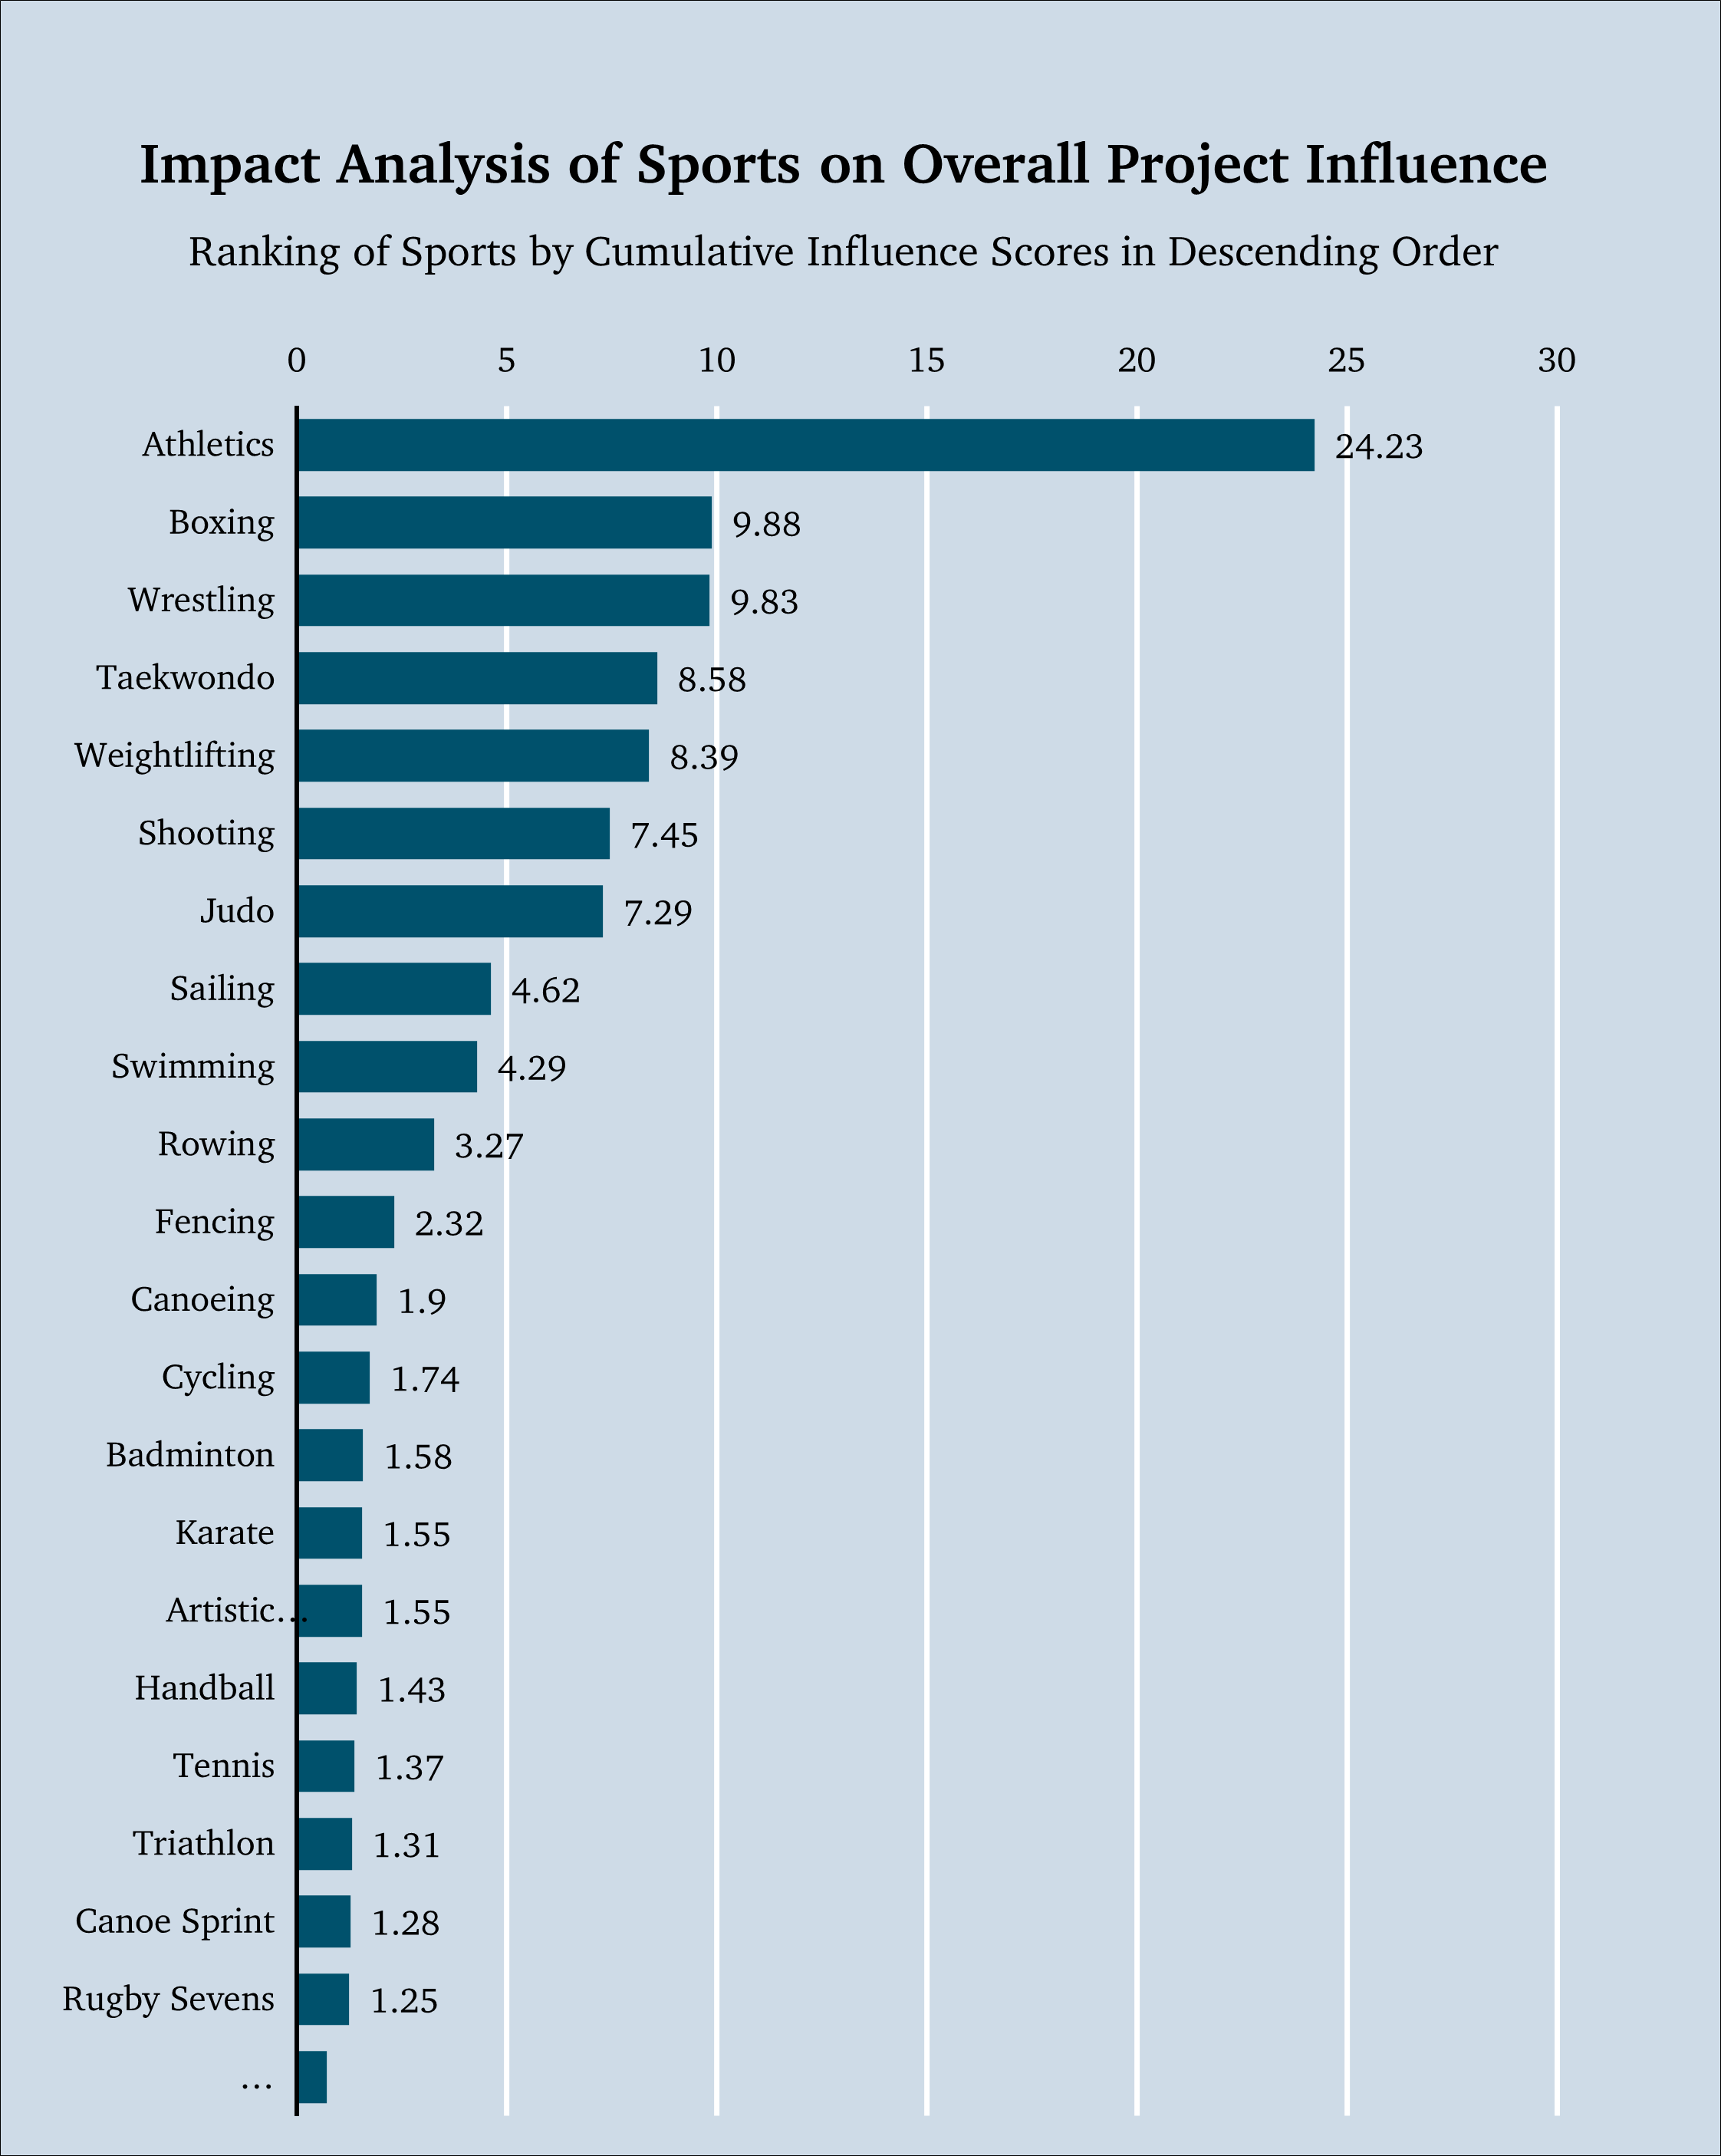
\includegraphics[width=0.48\textwidth]{pics/sport_influence_whole.png} % Reduced width for better fit
%     \caption{Ranking of sports by global importance based on aggregated event importance values across all countries.}
%     \label{fig:sport_importance}
% \end{wrapfigure}


\subsubsection{Results and Insights}
The analysis reveals that the importance of sports varies significantly across countries. The ranking of sports based on global importance highlights sports such as athletics, swimming, and gymnastics as the most influential globally. These sports typically feature a larger number of events and offer more medal opportunities, which contributes to their higher global importance.


% \subsubsection{Discussion and Recommendations(Optional)}
% \begin{itemize}
%     \item Focus on events with higher importance values$w_{i,j}$ for specific contexts.
%     \item Encourage diversification in participation.
%     \item Further analysis can include regional comparisons or investigate temporal trends.
% \end{itemize}


\subsection{Subtask 3.3 --- Impact of Events Chosen by Host Countries on Olympic Results}

Following these steps, we analyze the impact of events chosen by some major host countries on their Olympic results.

\paragraph{Categorization of Events for a Country}

Events are categorized into three types:
\begin{itemize}
    \item \textbf{New Events:} Events that the country participated in for the first time during the given Olympic Games. These are identified as events not entered by the country in the previous five cycles.
    \item \textbf{Dominant Events:} Events in which the country earned medals in two consecutive previous Olympic Games.
    \item \textbf{Normal Events:} All remaining events that do not fall into the above categories.
\end{itemize}

\paragraph{Analysis of Event Performance}

For each event type:
\begin{itemize}
    \item Calculate the total number of events ($X$) and medals won ($Y$) in each year across a 16-year period.
    \item Compute the yearly ratio as $\text{R} = Y / X$.
    \item Derive the Z-score for the host year compared to neighboring years using:$Z = \frac{\text{R}_{\text{host year}} - \mu}{\sigma}$
    where $\mu$ stands for mean ratio of neighboring years($\mu = \frac{\sum_{i=1}^{16} R_i}{16}$), and $\sigma$ stands for standard deviation($\sigma = \sqrt{\frac{\sum_{i=1}^{16} (R_i - \mu)^2}{16}}$).
    \item Determine if $Z > 1.96$, indicating statistical significance.
\end{itemize}

\paragraph{Application to Multiple Host Countries}

Applied the algorithm above to various host countries. Z-scores for new, dominant, and normal events are calculated for each host country to identify patterns in performance.

\subsubsection{Results and Comparative Insights}


\begin{wrapfigure}{r}{8cm}  %这是图文混排的环境
    \centering
    % 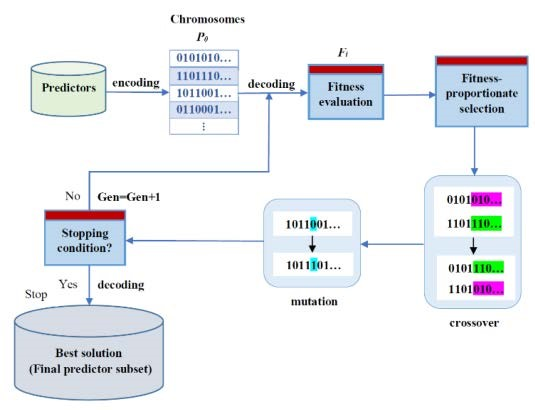
\includegraphics[width=0.9\linewidth,height=6cm]{pics/Multi-Agent_Optimization_Algorithm.jpg}
    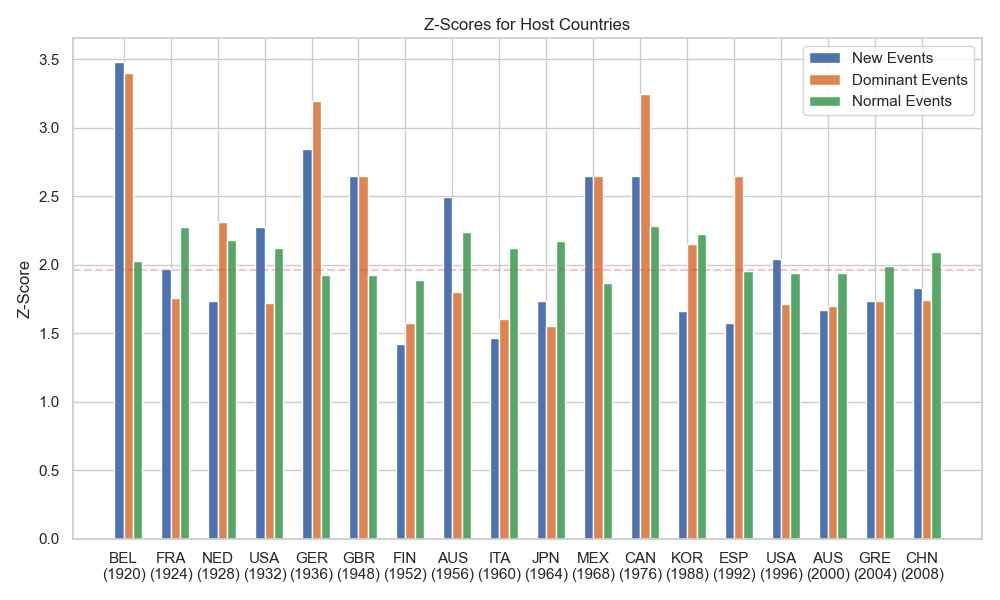
\includegraphics[width=0.5\textwidth]{pics/host_country_zscores.png}
    \caption{Comparison of Z-scores for new, dominant, and normal events across host countries.}
    \label{fig:zscore_comparison}
\end{wrapfigure}


\paragraph{Overall Trends Across Hosts}

Across 16 Olympic Games, the proportion of Z-scores exceeding 1.96 for each event category is:
\begin{itemize}
    \item \textbf{New Events:} 9 occurrences (56.25\%),
    \item \textbf{Dominant Events:} 8 occurrences (50.00\%),
    \item \textbf{Normal Events:} 11 occurrences (68.75\%).
\end{itemize}

\subsubsection{Conclusion}

The findings demonstrate that host countries rely most heavily on normal events to enhance their medal counts, with new events providing additional opportunities. Dominant events, while important, tend to show smaller incremental impacts, likely due to the high level of competition.


\section{Task2 --- The Great Coach Effect: its identification and impact}

The Great Coach Effect is a phenomenon where the presence of a highly skilled coach significantly improves the performance of athletes. Due to the fact that coaches are not bound to a specific country, they can have a significant impact on the medal counts of multiple nations. Identifying the Great Coach Effect and quantifying its impact on medal counts is crucial for predicting Olympic success.

\subsection{Identification}

\subsubsection{Methodology}

We reckon that the Great Coach Effect can be identified by comparing the performance of athletes under the same coach across different countries. It should, by nature, cause one country to have a sharp increase in their medal count in specific sports (otherwise this coach wouldn't be that great), and one other country to go through a gradual-to-sharp decrease in their medal count in the same sports. This is because the coach basically can only focus on coaching one country simultaneously, and the athletes from the other country would not receive the same level of training and support.

Again, due to the inherent limitation of usable dataset, we can only seek to identify the Great Coach Effect from this characteristic, rather than other methods such as relying on coach information to deduce the effect.

Therefore, we propose a two-step approach to identify and quantify the Great Coach Effect:

\begin{enumerate}
    \item Identify such pattern across the dataset.
    \item Refer to outside sources to interpret and cross-verify the result, finding out which specific coach is causing the effect each time.
\end{enumerate}

\subsubsection{Implementation}

We implemented the data filtering logic in Python with 0.23k LOC. The program reads the dataset, groups the data by country, sport, and year, and calculates the weighted medal count for each combination(gold medals with weight 3, silver with 2 and bronze with 1). It then uses linear regression on the most recent 12 years of data to calculate the slope of the medal trend over time. A positive slope exceeding a defined threshold (POS\_K\_LOWER) indicates a sharp increase, while a negative slope below another threshold (NEG\_K\_UPPER) indicates a gradual-to-sharp decrease. Countries with significant trends are recorded as having possible increases or decreases.

The program then pairs countries with overlapping trends in the same sport, checking the overlap period to ensure it spans at least four years and does not exceed a defined gap (OVERLAP\_GAP\_UPPER). Paired trends suggest the transfer of coaching expertise from one country to another.

By carefully calibrating the thresholds and gaps, we can effectively identify the Great Coach Effect and quantify its impact on national performances. We present the visual representation of the potential occurrences of the Great Coach Effect from both sport level and event level in \textit{Figure~\ref{fig:great_coach_effect}}.
\begin{figure}[htbp]
    \begin{minipage}[t]{0.5\textwidth}
        \centering
        \includegraphics[width=0.8\textwidth]{pics/great_coach_effect_analysis_(sport_level).png}
    \end{minipage}
    \begin{minipage}[t]{0.5\textwidth}
        \centering
        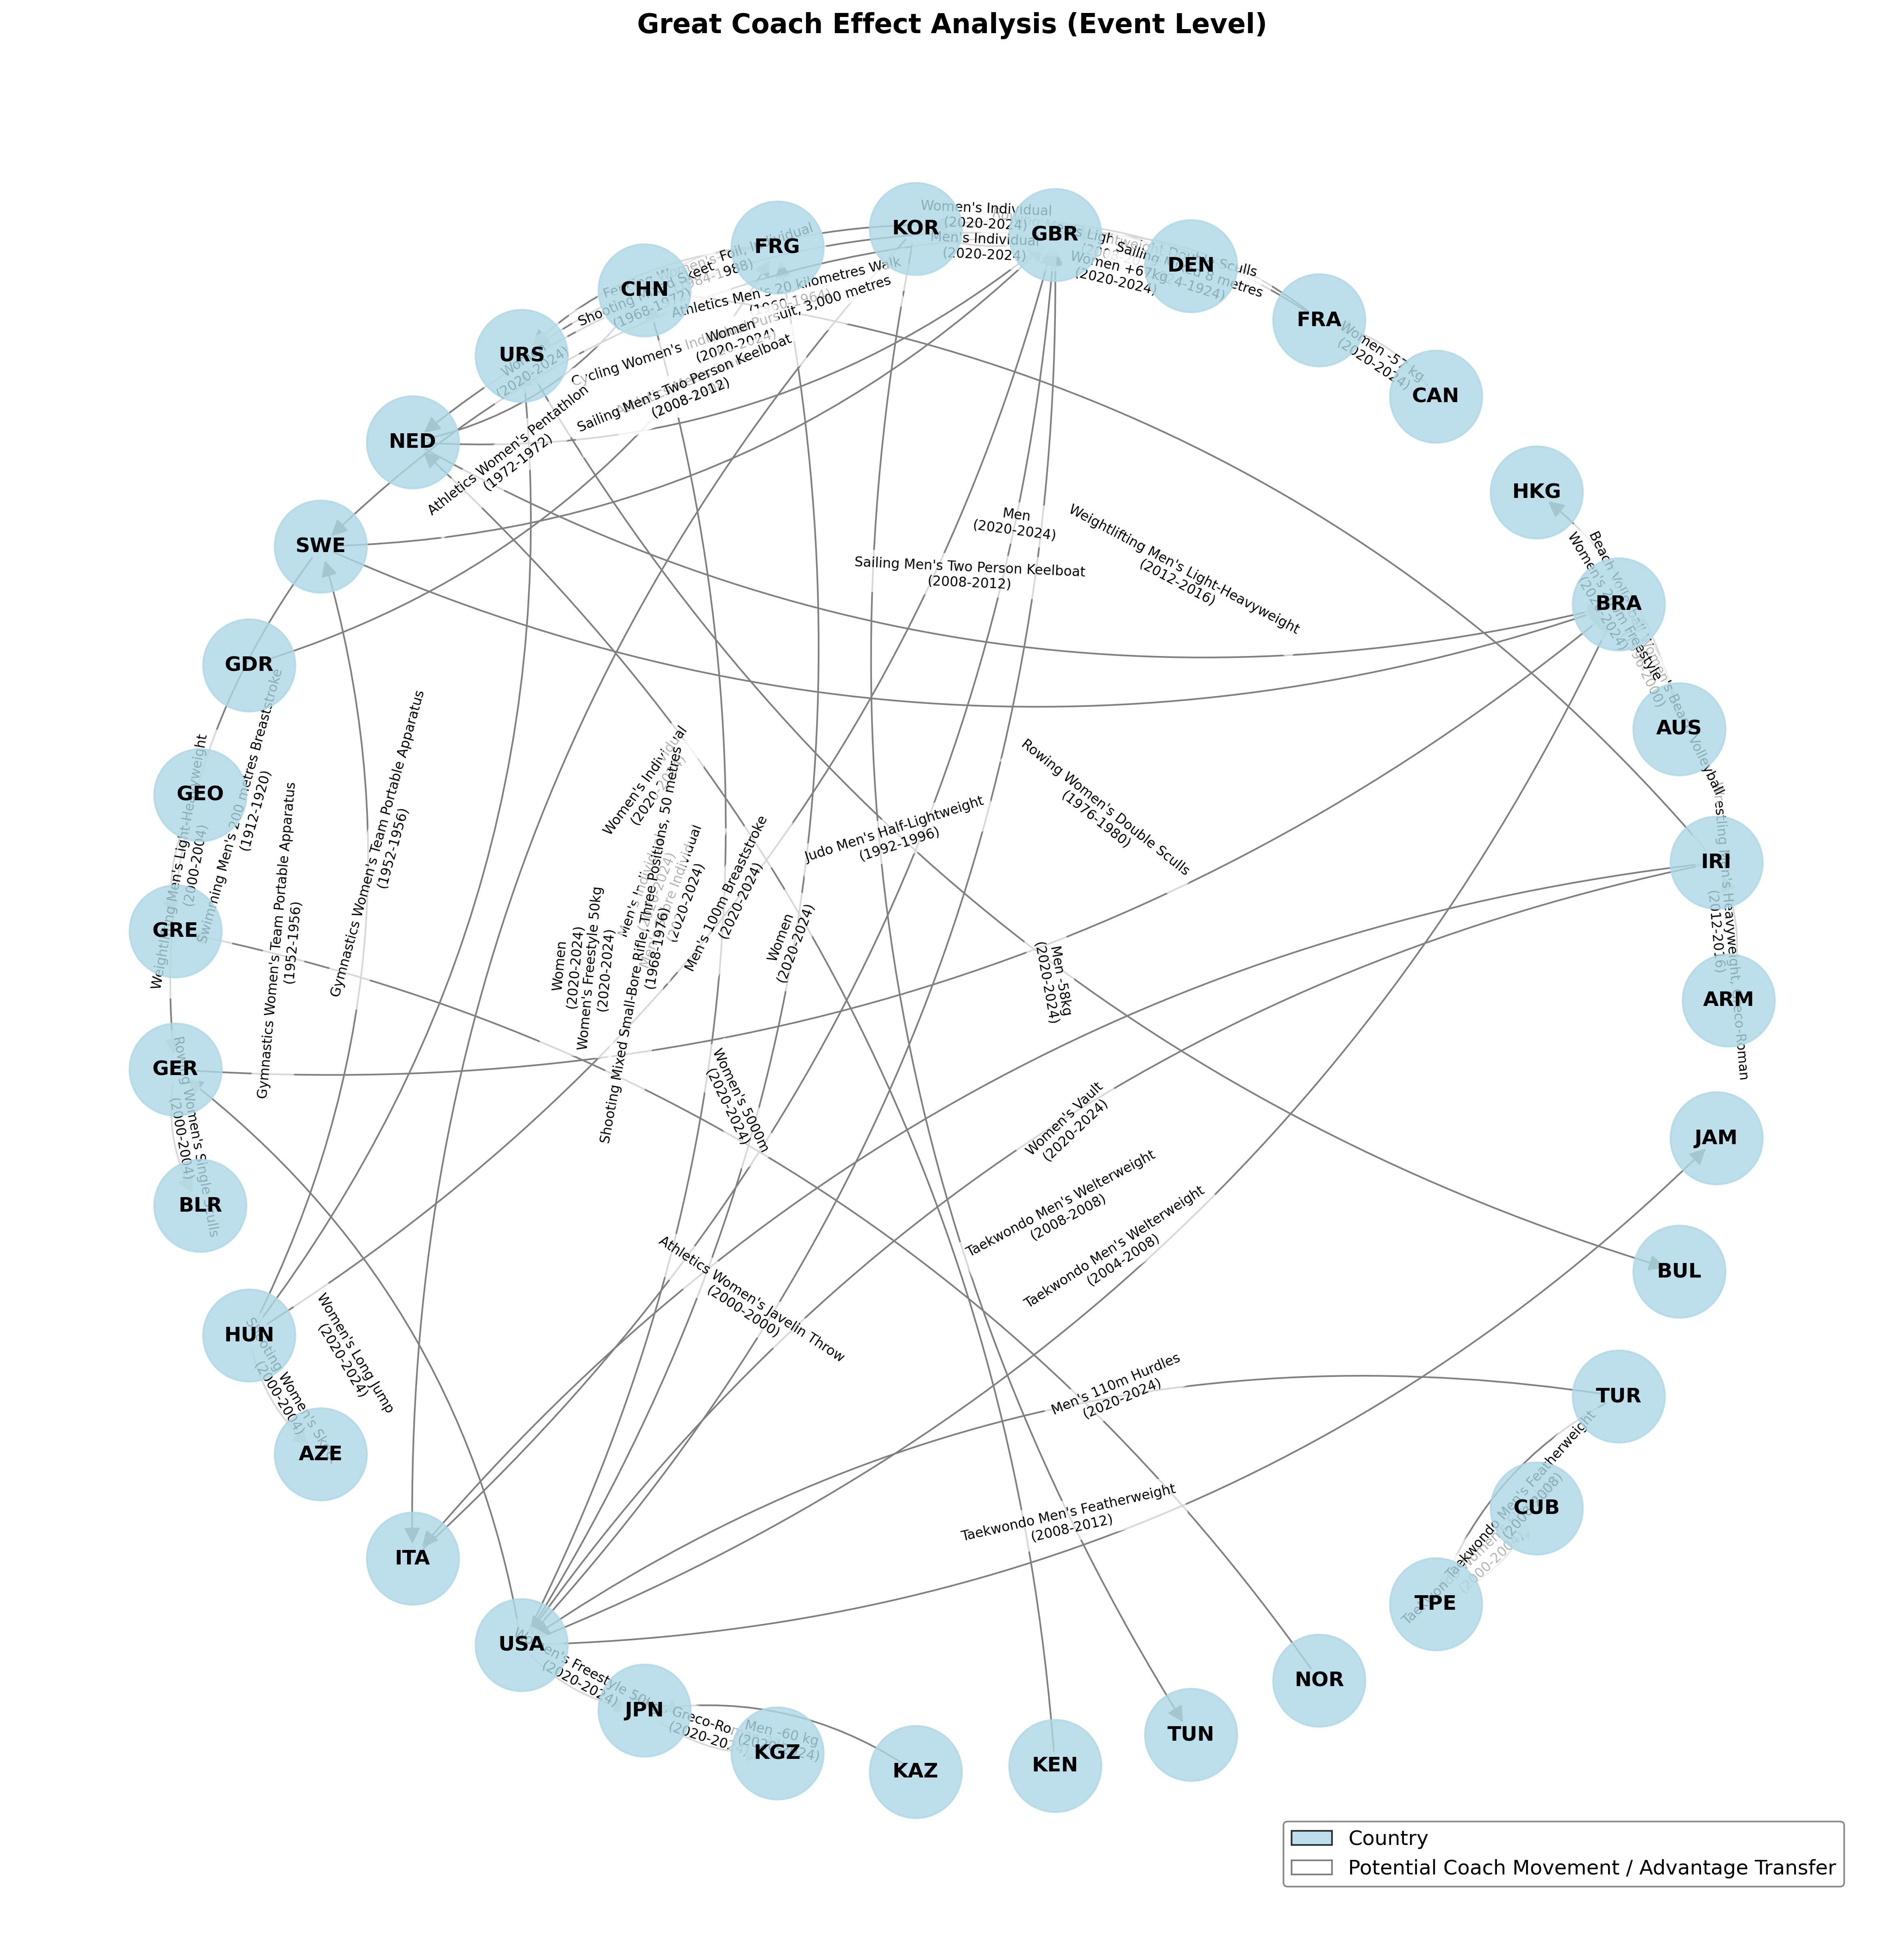
\includegraphics[width=0.8\textwidth]{pics/great_coach_effect_analysis_(event_level).png}
    \end{minipage}
    \caption{Potential occurences of The Great Coach Effects from sport level and event level}
    \label{fig:great_coach_effect}
\end{figure}

However elaborate we may calibrate the parameters, there still exists the issue of false positives and false negatives, with false positives accounting more because other factors may also contribute to this same characteristic. We recommend cross-referencing the results with external sources, such as coaching records and athlete interviews, to validate the findings and pinpoint the specific coaches responsible for these shifts. This data-driven approach allows for systematic identification of the Great Coach Effect, providing actionable insights into the strategic importance of coaching in achieving Olympic success.

\subsection{Quantification}

\subsubsection{Methodology}

We will quantify two main aspects of the Great Coach Effect: the magnitude of the performance change in both medal counts changes and the percentage of that change to the total medal count of the country.

The magnitude of the performance change can be calculated by comparing the average medal count before and after the coach transfer, while the percentage of the change can be calculated by dividing the change in medal count by the total medal count of the country in the respective sport.

These two aspects, especially the percentage of medal change to the total medal count of the country, have inextricable correlations with the overall strength of the country. Therefore, we will employ the same strategy as in our model establishment to cluster countries based on their historical medal counts, and then quantify the Great Coach Effect within each cluster.


\subsubsection{Implementation}

We further polish the program used in the identification step to calculate the magnitude and percentage of the Great Coach Effect, adding an additional 0.23k LOC. The program categorizes countries based on their tier value, calculates the average increase/decrease in medal count, and computes the average percentage of this change relative to the total medal count of the country. These metrics provide a comprehensive view of the Great Coach Effect's potential impact on different countries and sports.

\begin{figure}[htbp]
    \centering
    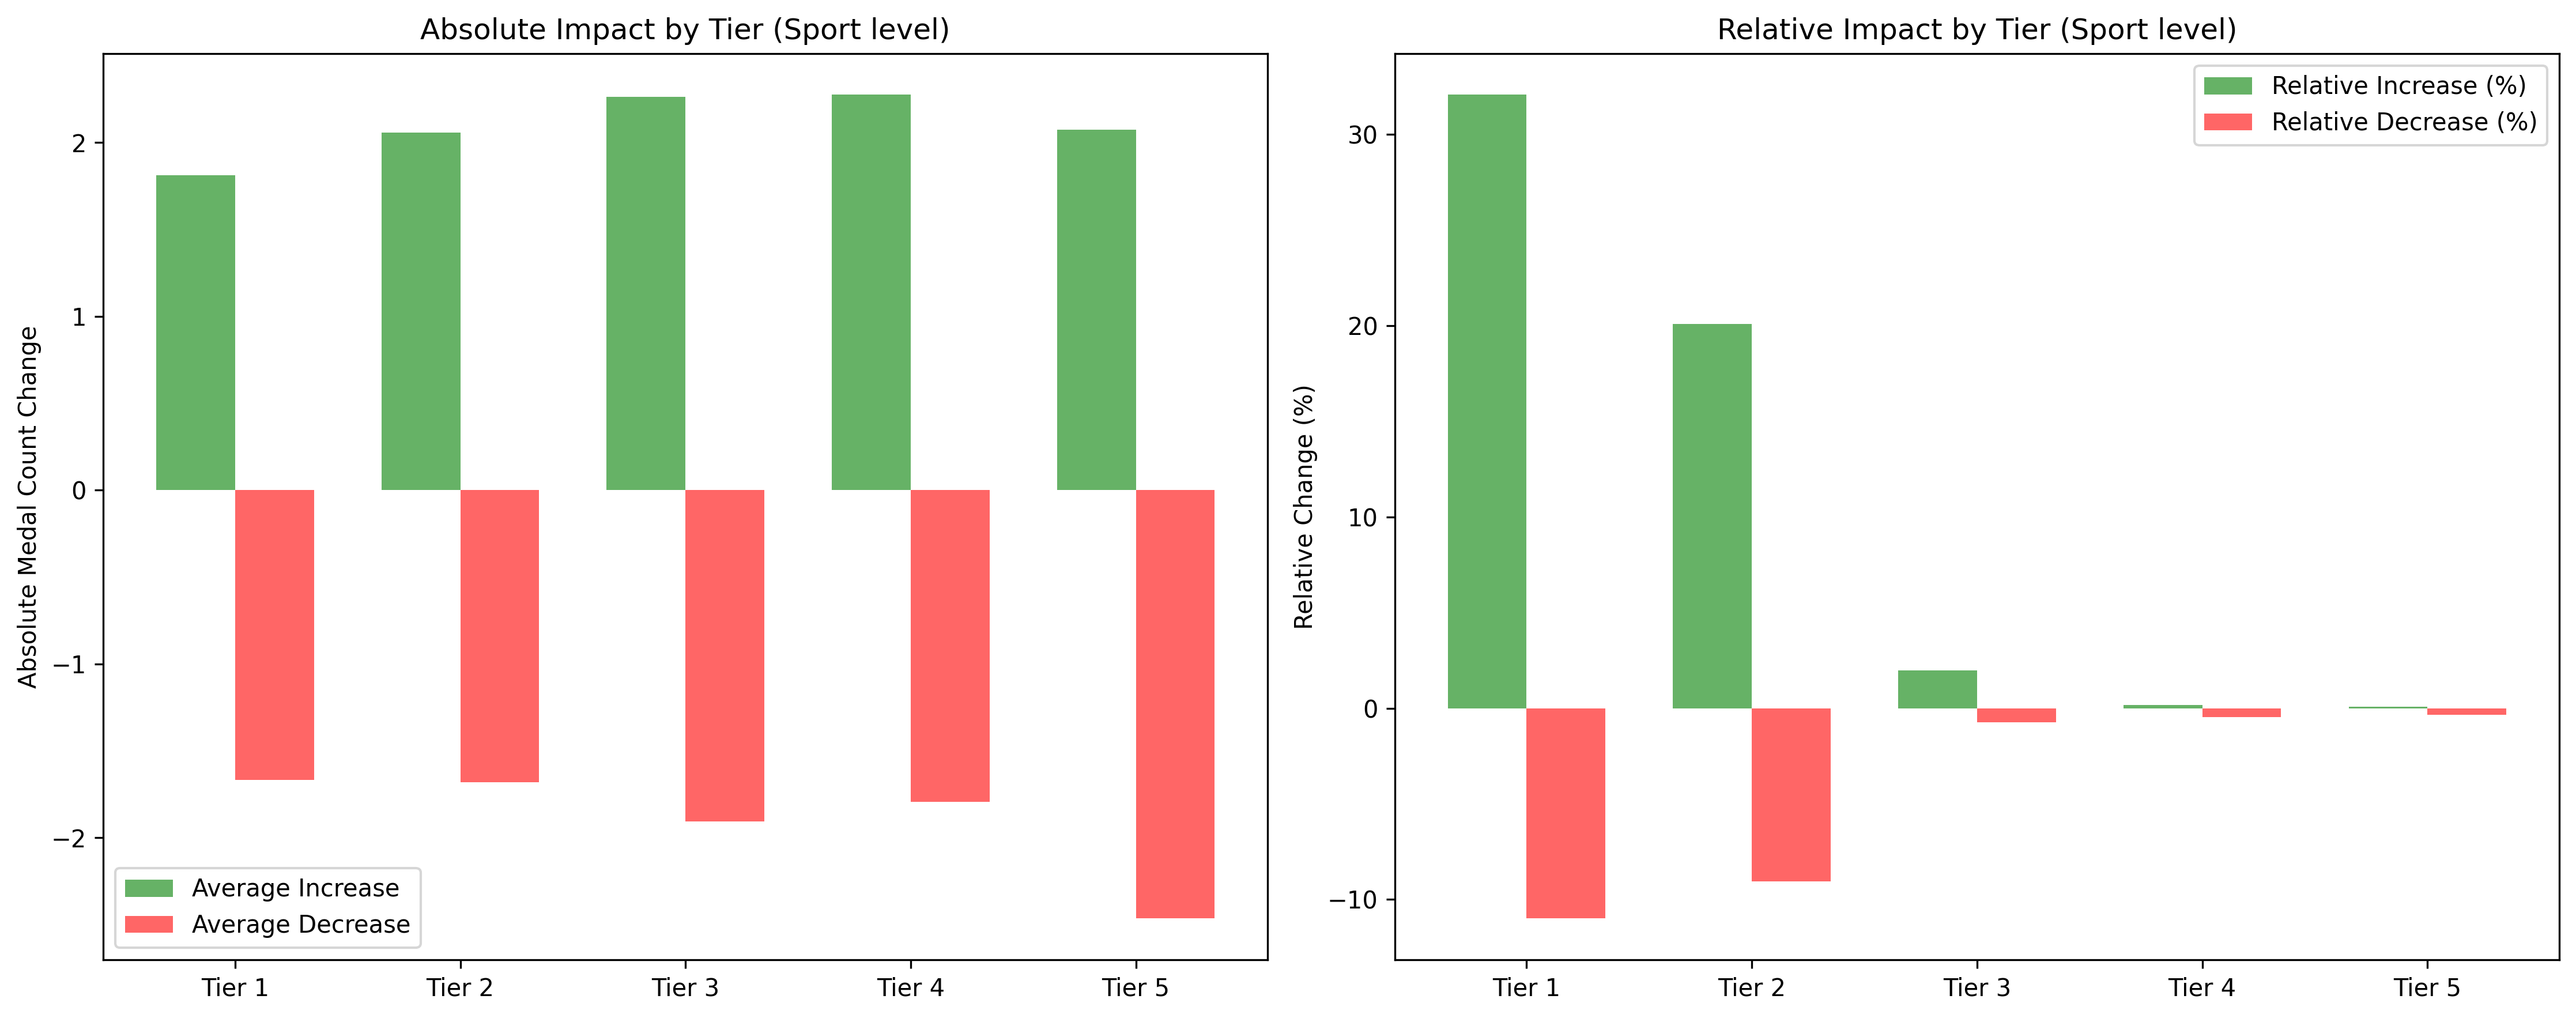
\includegraphics[width=0.8\textwidth]{pics/coach_effect_impact_Sport_from_csv.png}
    \caption{Quantification of The Great Coach Effect}
    \label{fig:coach_effect_impact}
\end{figure}

\begin{table}[htbp]
    \centering
    \begin{tabular}{|c|c|c|c|c|}
        \hline
        Tier & Avg. Increase & Avg. Decrease & Relative Increase(\%) & Relative Decrease(\%) \\
        \hline
        1 & 1.8125 & -1.6667 & 32.0772 & -10.9944 \\
        \hline
        2 & 2.0562 & -1.6795 & 20.1028 & -9.0563 \\
        \hline
        3 & 2.2623 & -1.9041 & 1.9766 & -0.7317 \\
        \hline
        4 & 2.2743 & -1.7923 & 0.1780 & -0.4518 \\
        \hline
        5 & 2.0746 & -2.4638 & 0.0660 & -0.3472 \\
        \hline
    \end{tabular}
    \caption{Impact of The Great Coach Effect on Different Tiers of Countries}
    \label{tab:coach_effect_impact}
\end{table}

\textit{Figure~\ref{fig:coach_effect_impact}} and \textit{Table~\ref{tab:coach_effect_impact}} clearly shows the impact of the Great Coach Effect on different tiers of countries, highlighting the potential for significant performance improvements under the guidance of elite coaches. We can see that the positive and negative impact of the Great Coach Effect(namely, the moving in and out of great coaches) on absolute medal changes has remained constant among different tiers of countries, while its impact on relative medal changes decreases as the tier goes up. This is an expected phenomenon because countries with better overall power already do well in sports across a wide range of fields, so the arrival or departure of one specific coach won't have much effect relative to the total medal count. By quantifying the magnitude and percentage of the effect, we can better understand the strategic value of investing in high-caliber coaching talent and its implications for national Olympic success.

\subsection{Exemplification}
By analyzing the performance trends in specific sports, we identified notable cases where the transfer of a coach coincided with a sharp increase in performance of one country and a decline or stagnation for another, allowing for the cross-verification of our algorithms. Below are three exemplifications of the Great Coach Effect based on historical Olympic data and their correlations with our results.\

It is worth mentioning that the data generated by the program above provides pairs of trends where one country's performance in a certain event increases significantly while another decreases over the same period of time. To spot such pattern, we assign each kind of medal with a value and apply linear regression to the data over a certain of range to get the slope, where a positive slope indicates improvement and vice versa.

\subsubsection{Synchronized Swimming Women's Team: Ana Tarré}
\begin{lstlisting}
- Event: Synchronized Swimming Women's Team, Overlap Years [2008-2012], Increase: CHN(slope=0.125) / Decrease: ESP(slope=-0.250)
\end{lstlisting}

This piece of data generated by the program reveals a significant overlap in performance trends between China (CHN) and Spain (ESP) during the period from 2008 to 2012. China's positive slope (0.125) and Spain's negative slope (-0.250) aligns well with Ana Tarré's transition from coaching Spain to China in 2012.

During Ana Tarré's tenure with Spain (1996–2012), the team gradually improved, earning higher medals, peaking with a Silver medal in 2008 and a Bronze in 2012. However, after she transitioned to coaching China in 2012, Spain had dropped out of the podium positions since then until 2024, while China experienced a gradual rise, achieving a series of Silver medals and finally a Gold medal in 2024, strongly aligning with the Great Coach Effect.

\subsubsection{Gymnastics Women's Team All-Around: Béla Károlyi}
\begin{lstlisting}
- Event: Gymnastics Women's Team All-Around, Overlap Years [2000-2008], Increase: USA(slope=0.125) / Decrease: ROU(slope=-0.250)
\end{lstlisting}

According to the program data, the overlap period between Romania (ROU) and the United States (USA) spans from 2000 to 2008. During this time, Romania exhibited a steep negative slope (-0.250), whereas the United States showed a positive one (0.125), which matches the historical narrative of Béla Károlyi's influence.

Béla Károlyi's legendary coaching career demonstrates a clear pattern of the Great Coach Effect. While coaching Romania (1974–1981), he elevated the team to global prominence, culminating in Silver medals in 1976 and 1980. After moving to coach the United States (1981–2016), Romania's performance declined, while the U.S. women's gymnastics team emerged as a dominant force.

\subsubsection{Women's Volleyball: Lang Ping}
\begin{lstlisting}
- Event: Volleyball Women's Volleyball, Overlap Years [1992-2004], Increase: CHN(slope=0.175) / Decrease: USA(slope=-0.075)
- Event: Volleyball Women's Volleyball, Overlap Years [2004-2012], Increase: USA(slope=0.250) / Decrease: CHN(slope=-0.375)
\end{lstlisting}

The program identifies two overlapping periods: 1992-2004 and 2004-2012. In both periods, one of CHN/USA rises and the other falls, which closely corresponds to Lang Ping's coaching career.

Looking at Lang Ping's coaching career spanning over 20 years, we can also discover the distinct influence of a capable coach. During her first tenure with China (1995-2005), the team achieved notable successes, including a Gold medal in 2004. After transitioning to coach the U.S. team (2005-2013) which had won few medals in history, U.S. quickly surpassed China and won 2 consecutive Silver medals. When Lang Ping returned to coach China in 2013, the Chinese team quickly regained its dominance with a Gold in 2016.

% These examples illustrate how the transfer of elite coaches can create significant shifts in medal performance across countries, substantiating the Great Coach Effect. The patterns not only validate the causality between coaching expertise and medal counts but also provide insights for national Olympic committees to consider investing in high-caliber coaching for sustained success.

\subsection{Recommendation}

In the Quantification part, we represented that the Great Coach Effect has a consistent impact on the absolute medal count changes across different tiers of countries, while its impact on relative medal count changes decreases as the tier goes up. This suggests that investing in elite coaching talent can yield substantial performance improvements, particularly for countries with lower historical medal counts(represented by low tier).

Therefore, we recommend that national Olympic committees prioritize recruiting and retaining top-tier coaches for tier 2 countries. Tier 1 countries usually have too tight a budget to afford the cost of coaches with great expertise, while it won't be really necessary for tier 3~5 countries to do so because of the low relative effect.

To determine which three tier 2 countries can benefit the most from the Great Coach Effect, we use the python code from Quantification part and modifies it to find the 3 countries with the highest potential for performance improvement. 

\begin{figure}[htbp]
    \centering
    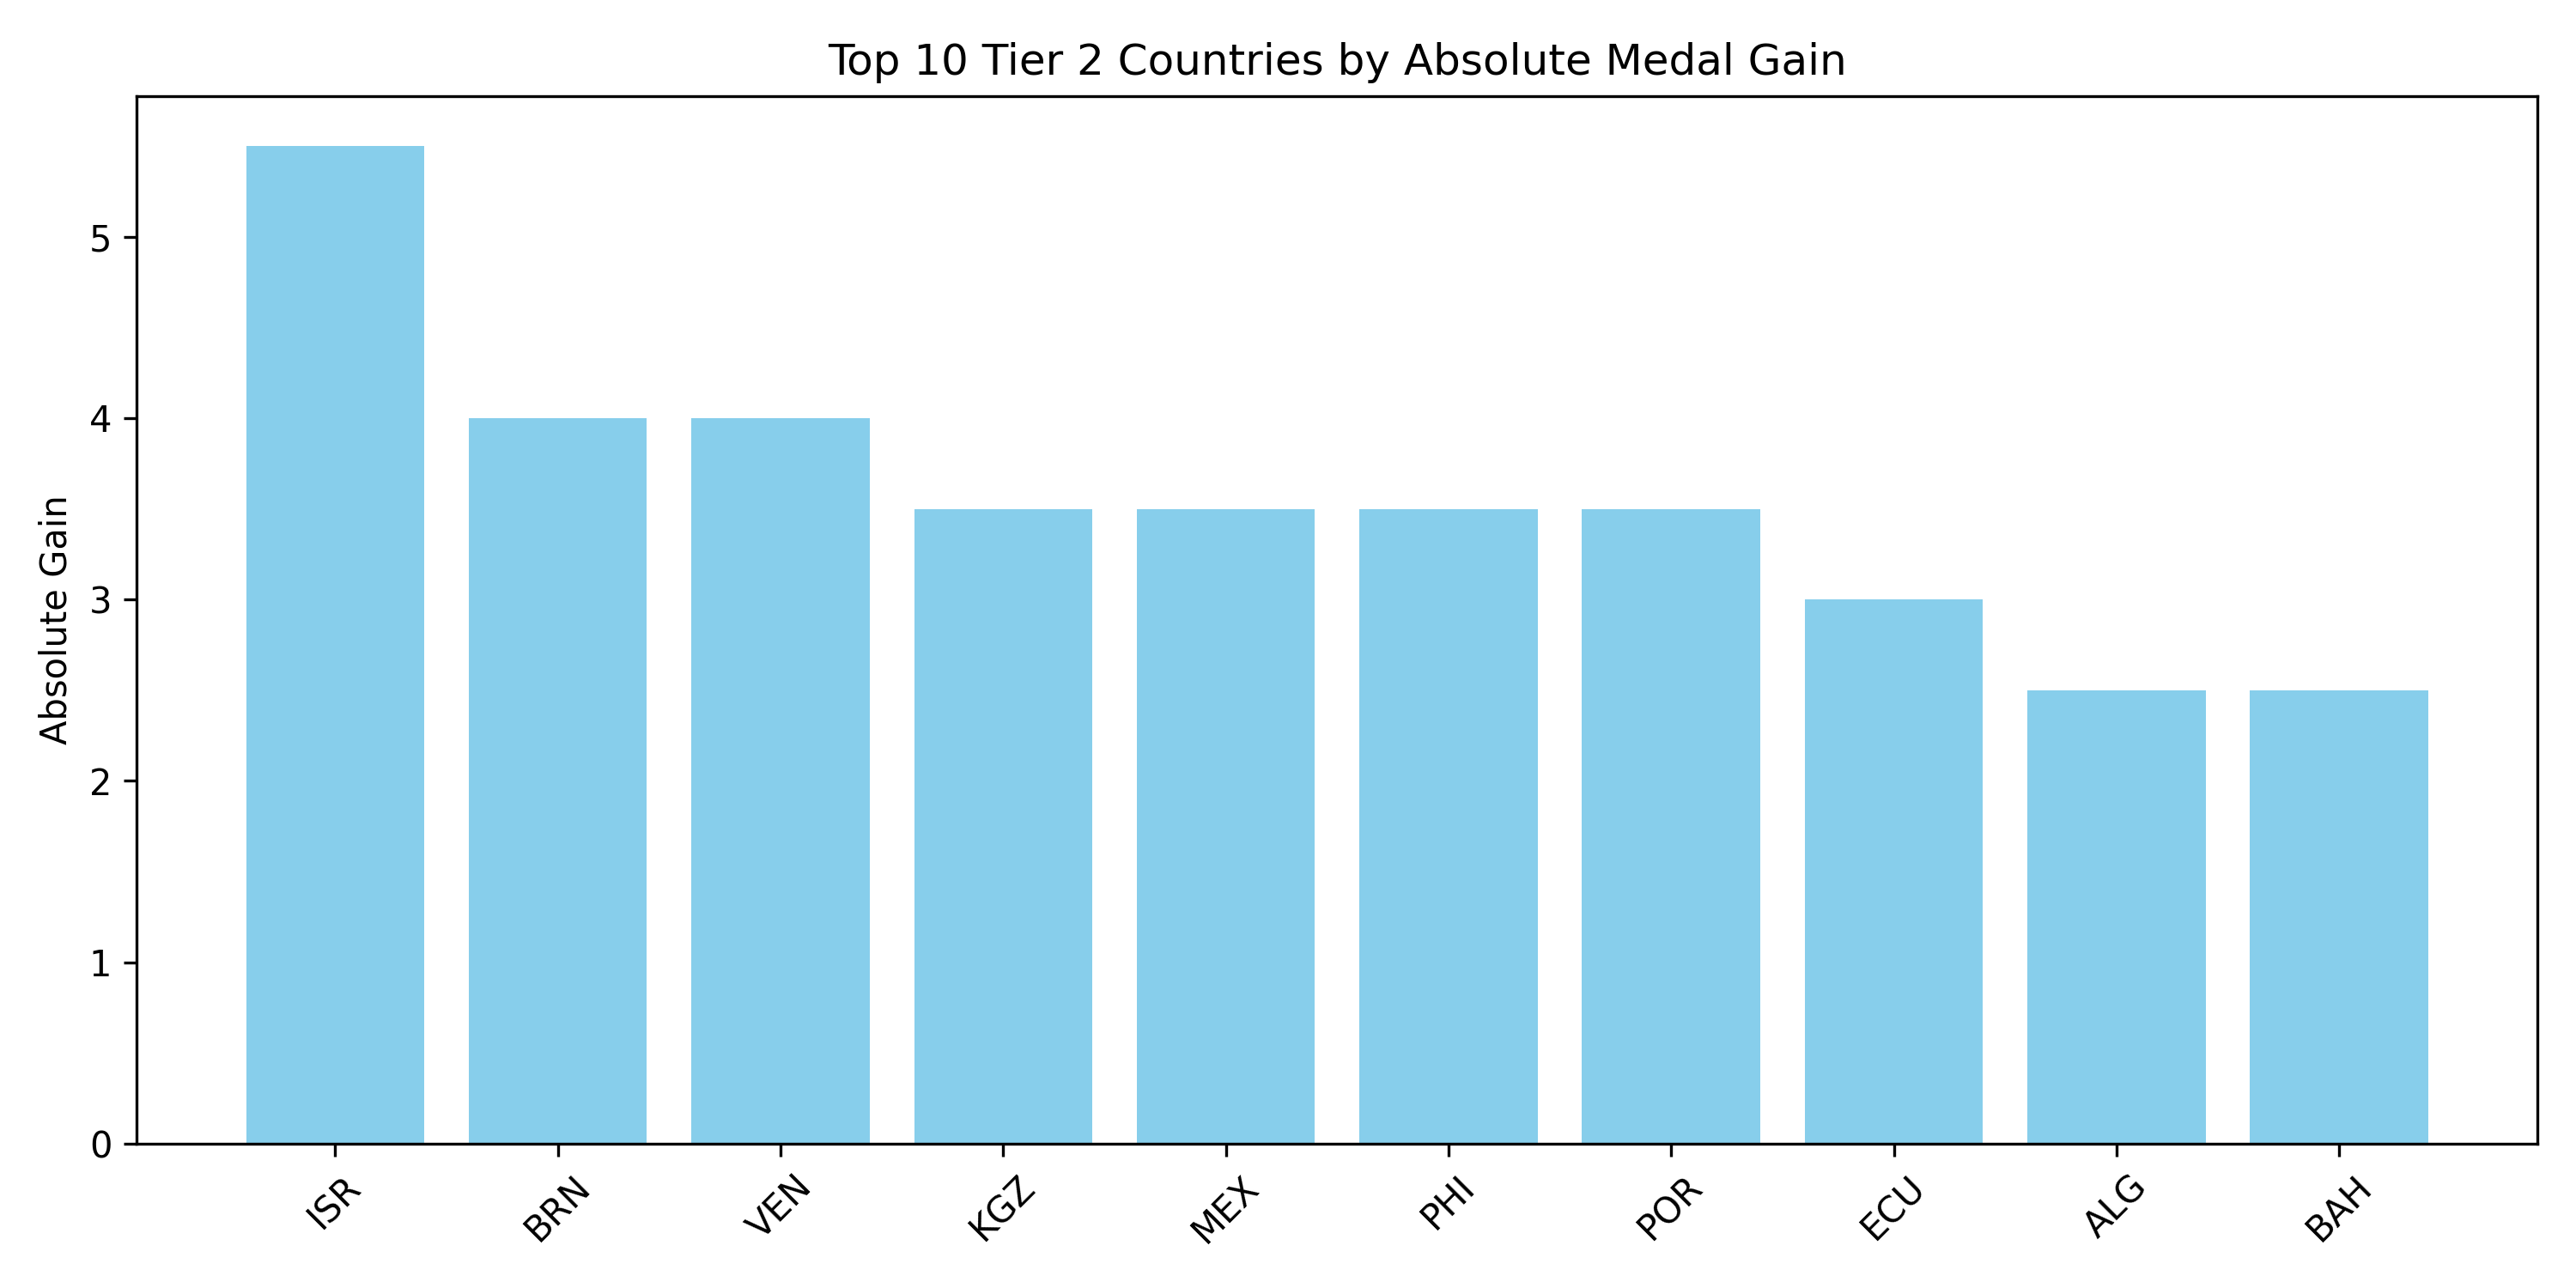
\includegraphics[width=0.8\textwidth]{pics/tier2_top10_absolute_gain.png}
    \caption{Quantification of The Great Coach Effect on Tier 2 Countries}
    \label{fig:tier2_top10_absolute_gain}
\end{figure}

As is shown in \textit{Figure~\ref{fig:tier2_top10_absolute_gain}}, we recommend the top 3 countries with the highest potential for performance improvement: ISR (Israel), BRN (Bahrain), and VEN (Venezuela), with respective projected medal gain of 5.5, 3.9 and 3.9.


\section{Task3 --- Original Insights revealed from the model}
\subsection{Global Sports Equity}
% 体育全球共有
In our analysis of the Great Coach Effect, we've shown that the impact of elite coaching talent can exert great influence on low-tier countries, assisting in the establishment of a more level playing field in the global sports arena and contributing to a more equitable global sports landscape.

We recommend that countries with elite coaches consider sharing their expertise with nations that have historically underperformed in those sports. This collaborative approach can elevate the global standard of competition, foster international goodwill, and ensure a more equitable distribution of knowledge and skills across the sporting world. By promoting a more inclusive and diverse competitive environment, we can enhance the global appeal and accessibility of various sports.


\subsection{Host Country Effect and Regulation}
% Host Country 显著 -> regulation限制
\begin{figure}[htbp]
    \centering
    \begin{minipage}[t]{0.45\linewidth}
        \centering
        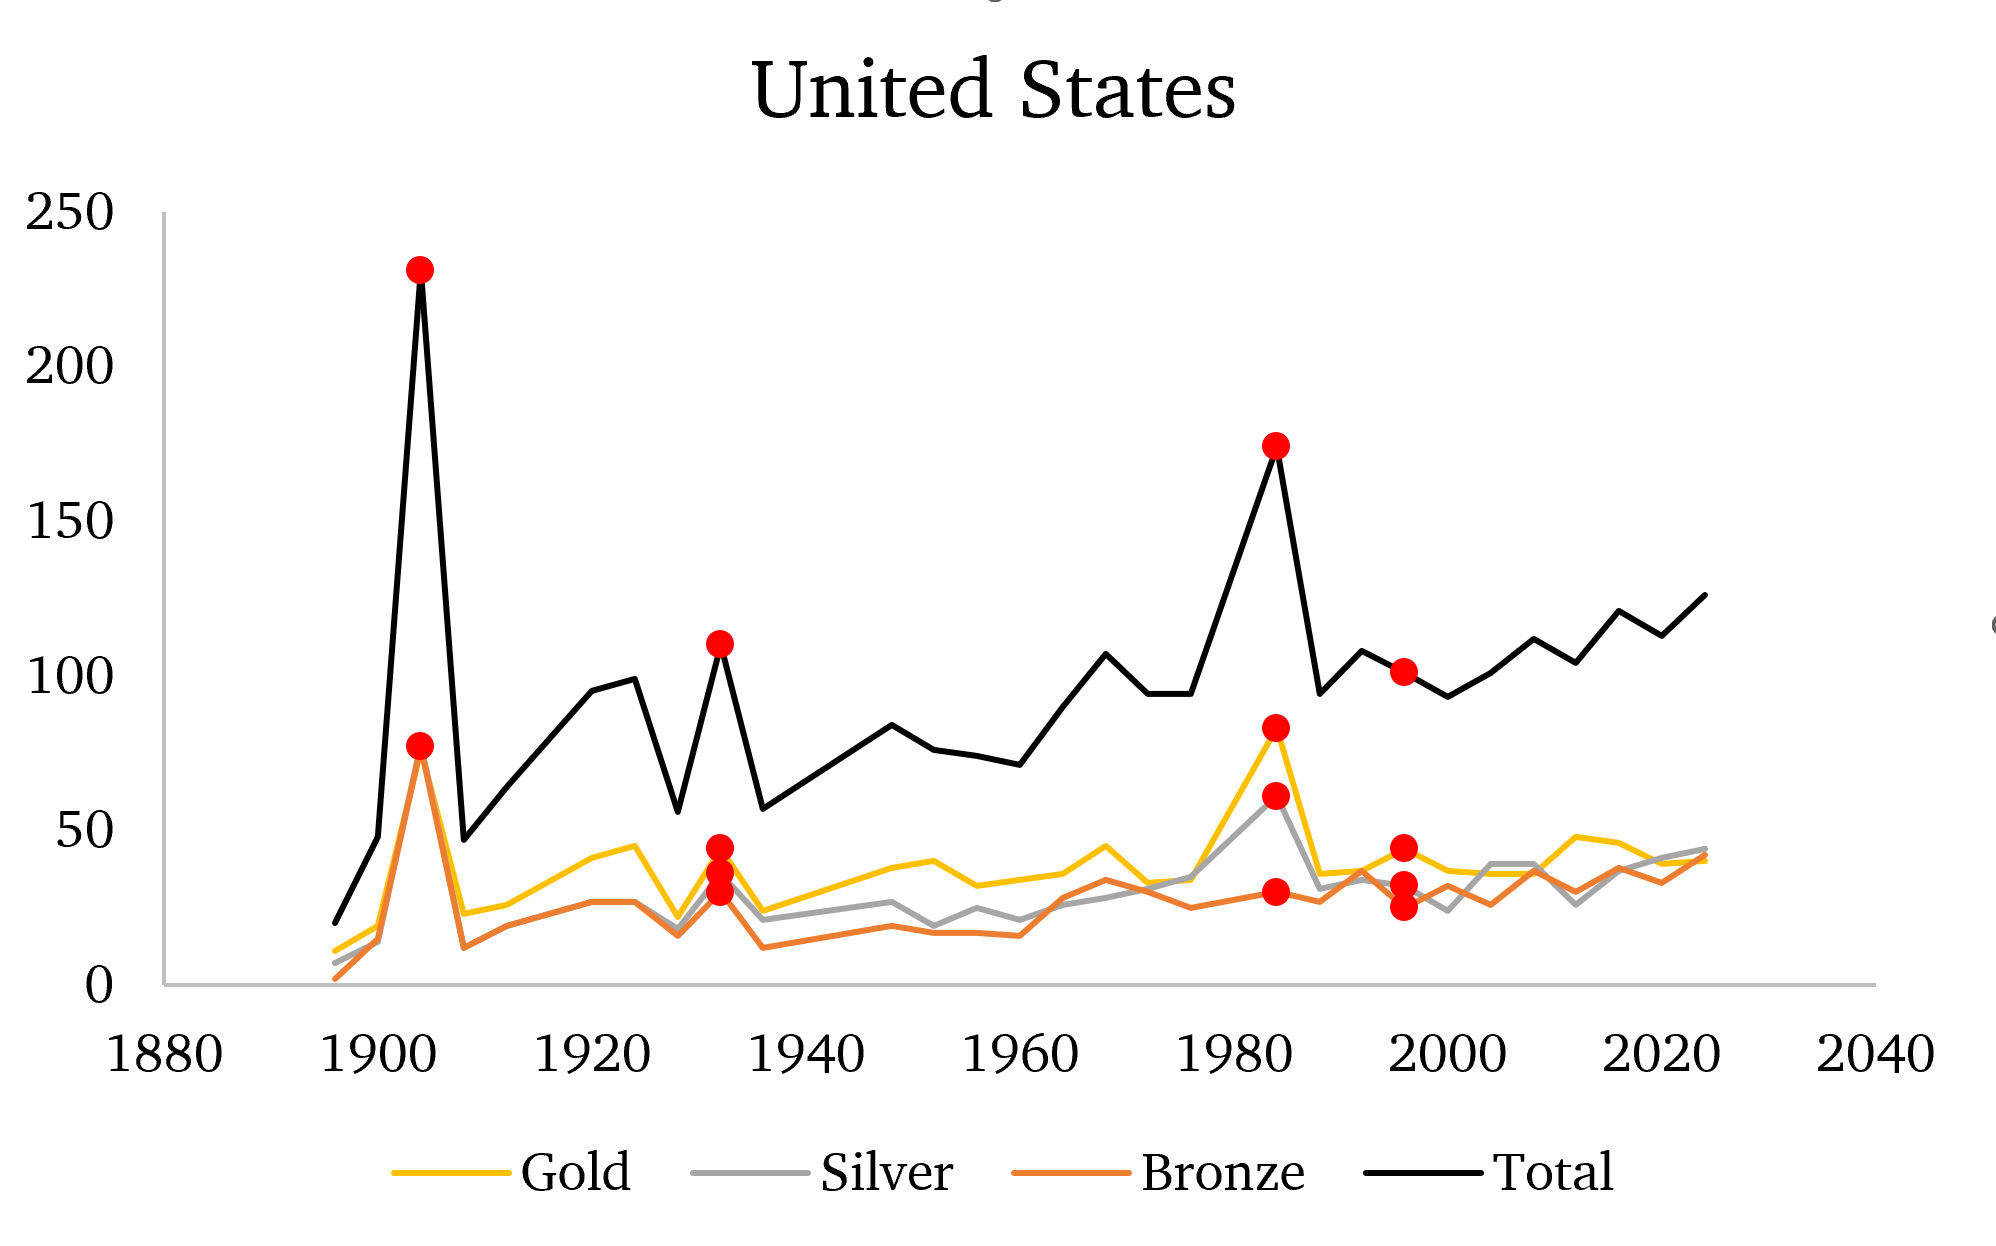
\includegraphics[width=8cm]{pics/USA.png}
        % \caption*{USA}
    \end{minipage}%
    \hfill
    \begin{minipage}[t]{0.45\linewidth}
        \centering
        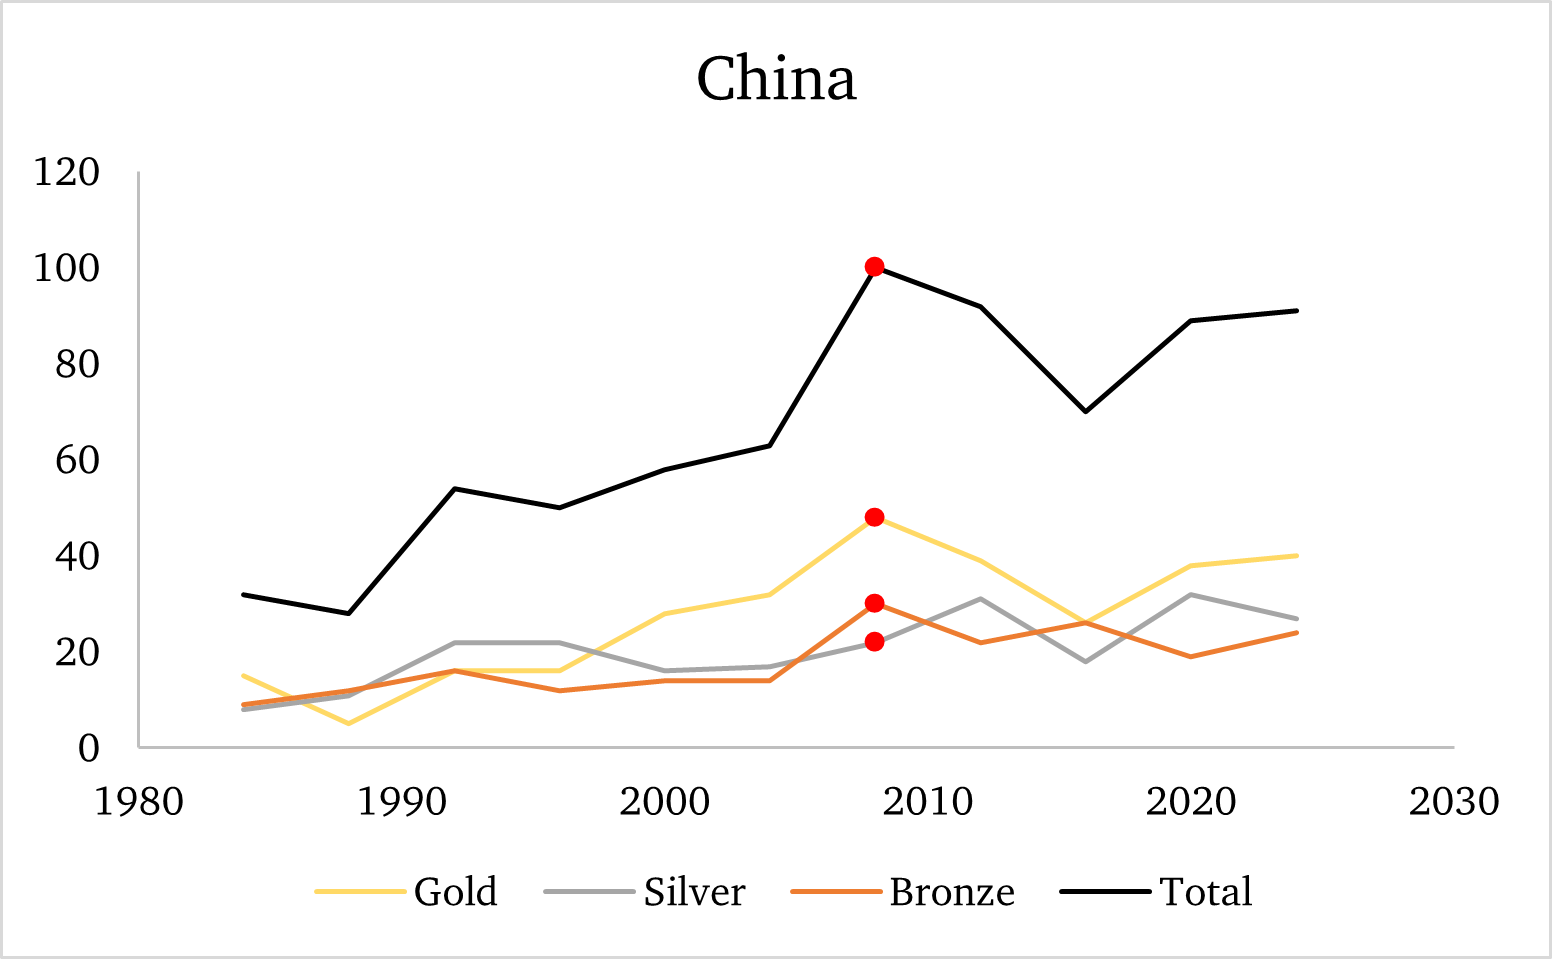
\includegraphics[width=8cm]{pics/CHN.png}
        % \caption*{CHN}
    \end{minipage}
    \caption{The Host-Country Effect on Medal Counts}
    \label{fig:host_country_effect}
\end{figure}


Analyzing the provided data, we observe a significant increase in medal counts for the United States during the years it hosted the Olympics: 1904, 1932, 1984, and 1996. For instance, in 1904, the US won 231 medals, a stark contrast to the 48 medals won in 1900. Similarly, China, as the host in 2008, saw a substantial increase in its medal count, winning 100 medals compared to 63 in 2004. This pattern suggests a strong host effect, where the host country benefits from factors such as home crowd support, familiarity with venues, and possibly more favorable conditions.

To curb such undesired host effects, regulations could be implemented to ensure a more level playing field. One approach could be to standardize training facilities and access for all participating countries well before the Games. Additionally, introducing stricter oversight on judging and scoring to prevent any potential bias towards the host nation can help. Another measure could be to limit the number of new events introduced by the host country, which might be tailored to their strengths. These regulations can help mitigate the host advantage, ensuring fairer competition and maintaining the integrity of the Olympic Games.

\subsection{Time-Sensitive Element in Prediction}
% NUMBER_OF_MATCHES 影响大 -> 时效性不好 -> ever changing
In our model evaluation part, we found that the number of matches immediately preceding the target year used to predict the outcome had a significant impact on the prediction performance. This suggests that the model's predictive power is highly sensitive to the number of matches played in the year leading up to the Olympics, strongly indicating that there is a time-sensitive element to the data.

Hence, we suggest that national Olympic committees and sports organizations pay close attention to the recent matches played in the year leading up to the Olympics. By monitoring and analyzing this data, they can gain valuable insights into the performance trends of athletes and teams, identify potential areas for improvement, and make informed decisions on training and preparation strategies. This time-sensitive element underscores the importance of adapting to ever-changing conditions and leveraging real-time data to optimize performance and maximize medal-winning opportunities.

% \subsection{}
% 不同时期增速不一致 -> 全球经济和政治状况 -> GDP/Total Medal


\subsection{Granularity Effect in Prediction Models}
Through our initial attempt at using individual athletes as the smallest granularity, we found that the model's prediction performance was significantly affected by the high randomness and variability in individual athlete performance and is thus defective.

In our initial attempt at using individual athletes as the smallest granularity, we found that the model's prediction performance was significantly affected by the high randomness and variability in individual athlete performance, making it defective.

This also reflects the real-world scenario, where allocating training resources to individual athletes is challenging due to the high uncertainty and variability in individual performance. Over-investing in a single project or athlete does not necessarily guarantee a return on investment, but in the meantime, taking part in more sports, as shown in the model, can steadily increase the chances of winning medals.

Therefore, we recommend that national Olympic committees focus on diversifying their participation in various sports to maximize their chances of winning medals. This strategy can help mitigate the risks associated with investing heavily in individual athletes and improve the overall performance of the country in the Olympics.

\section{Sensitivity Analysis}
In order to evaluate how changes in a key hyperparameter affect the overall prediction performance,
we perform a sensitivity analysis that varies the number of estimators for all the regression models we used.
Specifically, we adjust the \texttt{n\_estimators} parameter (if the model supports it) in the range of 25 to 175 with the step of 5, while maintaining consistent data and procedural steps otherwise.

We use 3-fold cross-validation on the same features and labels, and for each medal type
(\textit{Gold, Silver, Bronze}), we select the best performing model just as in the Model Evaluation part.
We compare each tested value against a baseline model where\texttt{n\_estimators}=100, calculating two proportions:
\begin{enumerate}
    \item \textbf{Inner\_param\_change\_proportion}: how much \texttt{n\_estimators} changes
    relative to the baseline, i.e. \(\frac{n\_value - 100}{100}\).
    \item \textbf{Result\_change\_proportion}: how much the average MAE changes
    relative to the MAE of the baseline, i.e. \(\frac{\text{MAE}(n\_value) - \text{MAE}(100)}{\text{MAE}(100)}\).
\end{enumerate}

\begin{figure}[htbp]
    \centering
    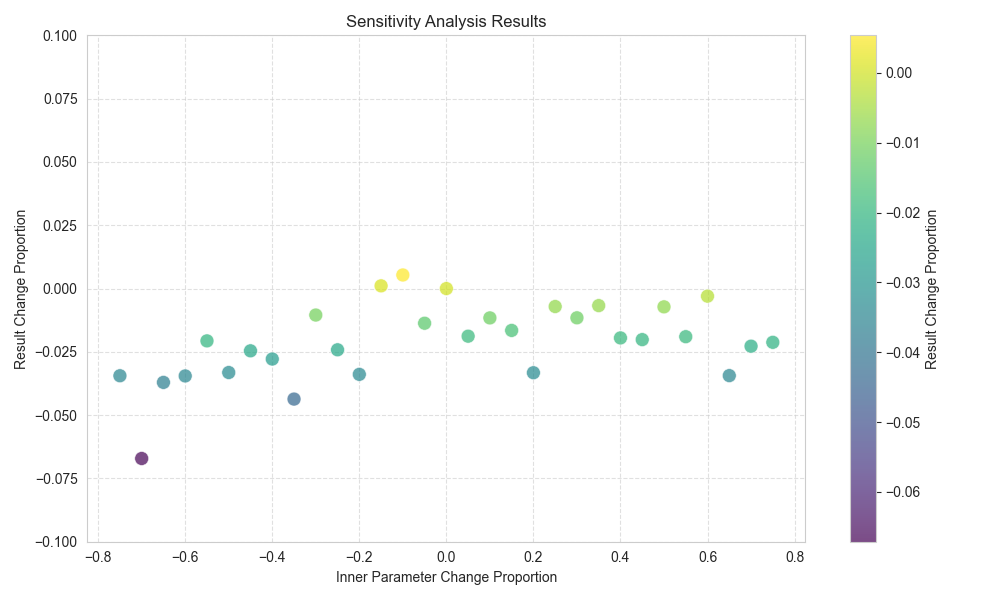
\includegraphics[width=0.8\textwidth]{pics/sensitivity_analysis.png}
    \caption{Sensitivity Analysis of the Number of Estimators}
    \label{fig:sensitivity_analysis}
\end{figure}

We can see from \textit{Figure~\ref{fig:sensitivity_analysis}} that the change in the number of estimators has a minor impact on the results overall, with the largest impact of them being only 7.5\%, and most of them around 2.5\%. This suggests that the model is relatively stable with respect to this hyperparameter, and the prediction performance is not significantly affected by the model parameters within the tested range.

\section{Conclusion}
In our work, we developed a comprehensive model to analyze and predict medal counts of 2028 Los Angeles Olympic Games, mainly focusing on historical performance, host country, and elite coaching. We quantified the "Great Coach Effect" and demonstrated its significant influence on medal counts. Our analysis revealed that investing in top-tier coaching talent can yield substantial performance improvements. Additionally, we examined the phenomenon of host countries experiencing a peak in medal counts during the hosting year, using Z-score analysis to quantify this effect. Our findings may provide valuable insights for national Olympic committees to strategically allocate resources and enhance their chances of success in future Olympic Games.

% AI cite use \AIcite{AI1,AI2,AI3}
\begin{thebibliography}{99}
    
    \bibitem{1} Ball, D. W. (1972). Olympic Games competition: Structural correlates of national success. International Journal of Comparative Sociology, 15, 186–200.
    \bibitem{2} Bernard, A. B., \& Busse, M. R. (2004). Who wins the Olympic Games: Economic resources and medal totals. Review of Economics and Statistics, 86, 414–417.
    \bibitem{3} Bian, X. (2005). Predicting Olympic Medal Counts: The Effects of Economic Development on Olympic Performance. The Park Place Economist, 13, 37-44.
    \bibitem{4} Forrest, D., Sanz, I., \& Tena, J. D. (2010). Forecasting national team medal totals at the Summer Olympic Games. International Journal of Forecasting, 26, 576–588.
    \bibitem{5} Schlembach, C., Schmidt, S. L., Schreyer, D., \& Wunderlich, L. (2022). Forecasting the Olympic medal distribution – A socioeconomic machine learning model. Technological Forecasting \& Social Change, 175, 121314.
    \bibitem{6} Tcha, M., \& Pershin, V. (2003). Reconsidering performance at the Summer Olympics and revealed comparative advantage. Journal of Sports Economics, 4, 216–239.
    \bibitem{7} Bernard A B, Busse M R. Who wins the Olympic Games: Economic resources and medal totals[J]. Review of economics and statistics, 2004, 86(1): 413-417.
    \bibitem{8} Xue, J., \& Shen, B. (2020). A novel swarm intelligence optimization approach: sparrow search algorithm. \textit{Systems Science \& Control Engineering, 8}(1), 22-34.
    \bibitem{9} Xue, J., \& Shen, B. (2023). Dung beetle optimizer: A new meta-heuristic algorithm for global optimization. \textit{The Journal of Supercomputing, 79}(7), 7305-7336.
    \bibitem{10} Mirjalili, S. (2016). SCA: a sine cosine algorithm for solving optimization problems. \textit{Knowledge-Based Systems, 96}, 120-133.
    \bibitem{11} Steinbrunn, M., Moerkotte, G., \& Kemper, A. (1997). Heuristic and randomized optimization for the join ordering problem. \textit{The VLDB Journal, 6}, 191-208.
    \bibitem{12} Zhan, Z. H., Zhang, J., Li, Y., \& Chung, H. S. H. (2009). Adaptive particle swarm optimization. \textit{IEEE Transactions on Systems, Man, and Cybernetics, Part B (Cybernetics), 39}(6), 1362-1381.
    \bibitem{13} Hashim, F. A., \& Hussien, A. G. (2022). Snake Optimizer: A novel meta-heuristic optimization algorithm. \textit{Knowledge-Based Systems, 242}, 108320.
    \bibitem{14} Trojovský, P., \& Dehghani, M. (2022). Pelican optimization algorithm: A novel nature-inspired algorithm for engineering applications. \textit{Sensors, 22}(3), 855.
    \bibitem{15} Mirjalili, S., Mirjalili, S. M., \& Lewis, A. (2014). Grey wolf optimizer. \textit{Advances in Engineering Software, 69}, 46-61.
\end{thebibliography}

% AI report begins here
\AImatter
\begin{ReportAiUse}{9}
\bibitem{AI1}
Github Copilot\\
Query1: make one elaborate plot out of this data:
1. add scatter points of year-country count
2. for the last 8 years [1996-2024], add the linear regression line onto the plot.

Output: I'll help you create a plot with scatter points and a linear regression line. Here's the solution step by step:

1. Import required libraries (numpy, pandas, matplotlib)

2. Read the CSV data

3. Create scatter plot for all points

4. Calculate and plot linear regression for the last 8 data points

5. Add labels and styling

Create a visualization script that plots the data with scatter points and regression line. [In main.py]

\begin{lstlisting}[language=python]
import pandas as pd
import numpy as np
import matplotlib.pyplot as plt
import seaborn as sns
from sklearn.linear_model import LinearRegression

# Read the CSV file
df = pd.read_csv('src/plot_1_2/summerOly_medal_country_count.csv')

# Set style
sns.set_style('whitegrid')
sns.set_palette("husl")

# Create figure
plt.figure(figsize=(12, 8))

# Plot all data points
sns.scatterplot(data=df, x='Year', y='Countries having earned medals',
                color='blue', alpha=0.6, label='Historical data')

# Get last 8 data points for regression
last_8 = df.tail(8)
X = last_8['Year'].values.reshape(-1, 1)
y = last_8['Countries having earned medals'].values

# Perform linear regression
reg = LinearRegression().fit(X, y)
y_pred = reg.predict(X)

# Create extended X range for prediction
X_extended = np.array([[x] for x in range(X.min()-4, 2033)])  # Extend before and after
y_extended = reg.predict(X_extended)

# Plot extended regression line
sns.lineplot(x=X_extended.flatten(), y=y_extended, color='red', linestyle='--',
             label=f'Linear trend (1996-2024)\nR² = {reg.score(X, y):.4f}')

# Add 2028 prediction point
prediction_2028 = reg.predict([[2028]])[0]
plt.scatter(2028, prediction_2028, color='red', s=35, zorder=5,
           label=f'2028 Prediction: {prediction_2028:.0f}')

# Customize the plot
plt.title('Cumulative Medal-Winning Countries by Olympic Year', 
          fontsize=18, pad=15)
plt.xlabel('Year', fontsize=12)
plt.ylabel('Number of Countries with Medals', fontsize=12)
plt.grid(True, alpha=0.3)
plt.legend(fontsize=10)

# Add text showing the regression equation
slope = reg.coef_[0]
intercept = reg.intercept_
equation = f'y = {slope:.2f}x {intercept:+.1f}'

# Calculate middle point of the regression line for text placement
mid_x = (X_extended.min() + X_extended.max()) / 2
mid_y = reg.predict([[mid_x]])[0]

# Place text horizontally above the regression line
plt.text(mid_x - 10, mid_y + 10, equation, 
         fontsize=18,
         verticalalignment='bottom',
         horizontalalignment='center',
         bbox=dict(facecolor='white', alpha=0.8, edgecolor='none'))

plt.tight_layout()
plt.show()

\end{lstlisting}

This script will create a plot showing:

1.Blue scatter points for all historical data

2.Red dashed line showing the linear regression for 1996-2024

3.Grid, labels, and legend

4.The regression equation and R² value

5.Modern styling with seaborn

6.The regression line will help visualize the trend in the number of countries earning medals in recent Olympics.

\bibitem{AI2}
Github Copilot

Query1: Insert Team\_or\_not and Team\_size as another two columns in the data frame.
Output: Sure, I can you with that. Here's the modified data frame:

\begin{lstlisting}
    Event, Team_or_not, Team_size
    10m Air Pistol Men, false, 1
    10m Air Pistol Mixed Team, true, 2
    10m Air Pistol Women, false, 1
    10m Air Rifle Men, false, 1
    10m Air Rifle Mixed Team, true, 2
    10m Air Rifle Women, false, 1
    25m Pistol Women, false, 1
    25m Rapid Fire Pistol Men, false, 1
    4 x 400m Relay Mixed, true, 4
    4 x 400m Relay Mixed Team, true, 4
    50m Rifle 3 Positions Men, false, 1
    50m Rifle 3 Positions Women, false, 1
    Aeronautics Mixed Aeronautics, false, 1
    Alpinism Mixed Alpinism, false, 1
    "Archery Men's Au Chapelet, 33 metres", false, 1
    "Archery Men's Au Chapelet, 50 metres", false, 1
    "Archery Men's Au Cordon Dore, 33 metres", false, 1
    "Archery Men's Au Cordon Dore, 50 metres", false, 1
    Archery Men's Championnat Du Monde, false, 1
    Archery Men's Continental Style, false, 1
    Archery Men's Double American Round, false, 1
    Archery Men's Double York Round, false, 1
    Archery Men's Individual, false, 1
    "Archery Men's Pole Archery, Large Birds, Individual", false, 1
    "Archery Men's Pole Archery, Large Birds, Team", true, 4
    "Archery Men's Pole Archery, Small Birds, Individual", false, 1
    "Archery Men's Pole Archery, Small Birds, Team", true, 4
    Archery Men's Sur La Perche a La Herse, false, 1
    Archery Men's Sur La Perche a La Pyramide, false, 1
    "Archery Men's Target Archery, 28 metres, Individual", false, 1
    "Archery Men's Target Archery, 28 metres, Team", true, 4
    "Archery Men's Target Archery, 33 metres, Individual", false, 1
    "Archery Men's Target Archery, 33 metres, Team", true, 4
    "Archery Men's Target Archery, 50 metres, Individual", false, 1
    "Archery Men's Target Archery, 50 metres, Team", true, 4
    Archery Men's Team, true, 4
    Archery Men's Team Round, true, 4
    Archery Men's Unknown Event, false, 1
    Archery Women's Double Columbia Round, false, 1
    Archery Women's Double National Round, false, 1
    Archery Women's Individual, false, 1
    ...
    "Wrestling Men's Super-Heavyweight, Greco-Roman", false, 1
    "Wrestling Men's Unlimited Class, Greco-Roman", false, 1
    "Wrestling Men's Welterweight, Freestyle", false, 1
    "Wrestling Men's Welterweight, Greco-Roman", false, 1
    "Wrestling Women's Featherweight, Freestyle", false, 1
    "Wrestling Women's Flyweight, Freestyle", false, 1
    "Wrestling Women's Heavyweight, Freestyle", false, 1
    "Wrestling Women's Light-Heavyweight, Freestyle", false, 1
    "Wrestling Women's Lightweight, Freestyle", false, 1
    "Wrestling Women's Middleweight, Freestyle", false, 1
\end{lstlisting}

\end{ReportAiUse}

\end{document}
